%!TEX program = xelatex
\documentclass[aspectratio=43,UTF8,10pt]{ctexbeamer}

    \mode<presentation> {
    \usetheme{Madrid}
    %\setbeamertemplate{footline} % To remove the footer line in all slides uncomment this line
    \setbeamertemplate{footline}[frame number] % To replace the footer line in all slides with a simple slide count uncomment this line
    \setbeamercolor{page number in head/foot}{fg=blue}
    \setbeamertemplate{navigation symbols}{} % To remove the navigation symbols from the bottom of all slides uncomment this line
    }

    % \usepackage[UTF8,noindent]{ctexcap} %使用ctexcap
    \usepackage{indentfirst}
    \setlength{\parindent}{2em}
    \usepackage{listings}
    % \lstset{extendedchars=false}%这一条命令可以解决代码跨页时,章节标题,页眉等汉字不显示的问题
    \lstset{language=C++, showstringspaces=false, basicstyle=\small}
    % \usepackage{fontspec}
    % \usepackage{ctex}
    \usepackage{xcolor,color}
    \usepackage{float}
    \usepackage{wrapfig}
    \usepackage{picinpar}
    \usepackage{graphicx}
    \usepackage{animate}
    \usepackage{tabularx}
    \usepackage{multicol}
    % \usepackage{movie15}
    \definecolor{indiagreen}{rgb}{0.07, 0.53, 0.03}
    \definecolor{indianred}{rgb}{0.8, 0.36, 0.36}
    \definecolor{indianyellow}{rgb}{0.89, 0.66, 0.34}
    \definecolor{bondiblue}{rgb}{0.0, 0.58, 0.71}
    \definecolor{ao(english)}{rgb}{0.0, 0.5, 0.0}
    \definecolor{azure(colorwheel)}{rgb}{0.0, 0.5, 1.0}
    % User Defined Block %%%%%%%%%%%%%%%%%%%%%%%%%%%%%%%%%%%%%%%%%%%%%%%%%%%%%%%%
    \newenvironment<>{abstractblock}[1]{%
      \setbeamercolor{block title}{fg=white,bg=bondiblue}%
    %   \setbeamercolor{block body}{fg=white,bg=bondiblue}%
      \begin{block}#2{#1}}{\end{block}}

    \newenvironment<>{thinkblock}[1]{%
      \setbeamercolor{block title}{fg=white,bg=azure(colorwheel)}%
    %   \setbeamercolor{block body}{fg=white,bg=bondiblue}%
      \begin{block}#2{#1}}{\end{block}}

    \newenvironment<>{yellowblock}[1]{%
      \setbeamercolor{block title}{fg=white,bg=indianyellow}%
      \begin{block}#2{#1}}{\end{block}}

    \lstset{language=C++,
    columns=flexible,
    basicstyle=\footnotesize\ttfamily,                                    % 设定代码字体、大小
    %numbers=left,xleftmargin=2em,framexleftmargin=2em,                   % 在左侧显示行号
    %numberstyle=\color{darkgray},                                        % 设定行号格式
    keywordstyle=\color{blue},                                            % 设定关键字格式
    commentstyle=\color{ao(english)},                                     % 设置代码注释的格式
    stringstyle=\color{brown},                                            % 设置字符串格式
    showstringspaces=false,                                              % 控制是否显示空格
    %frame=single,                                                         % 控制外框
    breaklines,                                                           % 控制是否折行
    postbreak=\space,                                                     % 控制折行后显示的标识字符
    breakindent=5pt,                                                      % 控制折行后缩进数量
    emph={size\_t,array,deque,list,map,queue,set,stack,vector,string,pair,tuple,ostream}, % 非内置类型
    emphstyle={\color{teal}},
    escapeinside={(*@}{@*)},
}


    \title
        % [第4章~复合类型、\texttt{string}和\texttt{vector}\hspace{2em}]
        {第4章~复合类型、\texttt{string}和\texttt{vector}}

%\author[李长河]{李长河} % Your name
%\institute[CUG] % Your institution as it will appear on the bottom of every slide, may be shorthand to save space
%{
%中国地质大学(武汉)\\ % Your institution for the title page
%\medskip
%\textit{lichanghe@cug.edu.cn} % Your email address
%}
\date{} % Date, can be changed to a custom date

\begin{document}

\maketitle


\begin{frame}{目录}
\begin{multicols}{2}
	\tableofcontents
\end{multicols}
\end{frame}

\begin{frame}{~}
	\begin{yellowblock}{学习目标}
		\begin{itemize}
			\item 理解指针和引用的工作机理;
			\item 掌握指针、引用和数组的使用方法;
			\item 理解指针与数组的关系,能够运用指针访问数组元素;
			\item 学会运用数组、\texttt{string}~和~\texttt{vector}~解决实际问题。
		\end{itemize}
	\end{yellowblock}
\end{frame}

\section{引用}
\subsection{左值引用}
\begin{frame}
	\frametitle{4.1 引用}
	\begin{block}{复合类型}
		复合类型是指基于其它类型定义的类型,包括指针、引用、数组、函数、类、联合体和枚举类型等
	\end{block}
	\begin{abstractblock}{引用}
		\begin{itemize}
			\item 为已创建的对象取一个\alert{别名}
			\item 只将别名绑定到所引用的对象,对象的内容不会复制给引用
			\item 函数间共享局部对象的重要途径,对于提高程序的效率有重要作用
		\end{itemize}
	\end{abstractblock}

	\begin{yellowblock}{说明:}
		C++11引入了右值引用,如无提示,引用默认为左值引用
	\end{yellowblock}

\end{frame}

\begin{frame}[fragile]
	{4.1 引用}
	\begin{block}{引用语法格式:}
		\begin{lstlisting}[basicstyle=\small\ttfamily]
int counter = 0;
int &refCnt = counter;  //refCnt引用counter对象的内容
int &refCnt2;             //错误:定义引用时必须和一个对象绑定
        \end{lstlisting}
		\begin{lstlisting}[basicstyle=\small\ttfamily]
refCnt = 2;       //修改了counter所在的内存空间的内容
int i = refCnt;//通过引用读取counter对象的内容,并初始化对象i
        \end{lstlisting}
	\end{block}
	\begin{alertblock}{建议:}
		书写上,把\textcolor[rgb]{1,0,0}{引用符号与对象名放在一起},而不是把类型名和引用符号放在一起,这样有助于\textcolor[rgb]{1,0,0}{提高程序的可读性}。如:\\
		\begin{lstlisting}[basicstyle=\small\ttfamily]
int counter = 0;
int& refCnt = counter;
    \end{lstlisting}
	\end{alertblock}
\end{frame}

\begin{frame}[fragile]
	{4.1 引用}
	\noindent 定义引用时,除了需要初始化外,还需要注意以下几点:
	\begin{block}{1. 定义多个引用时,每个引用必须用~\texttt{\&}~标明:}
		\begin{lstlisting}[basicstyle=\small\ttfamily]
int i = 0;
int &r1 = i, j = 0, &r2 = r1; //r1 和 r2 都是 i 的引用,而 j 是 int 类型
            \end{lstlisting}
	\end{block}
	\begin{block}{2. 只能引用同类型的对象:}
		\begin{lstlisting}[basicstyle=\small\ttfamily]
double d = 0;
int &r3 = d; //错误:r3 只能引用 int 类型对象
            \end{lstlisting}
	\end{block}
	\begin{block}{3. 引用的对象必须是非\texttt{const}左值:}
		\begin{lstlisting}[basicstyle=\small\ttfamily]
int i = 0; const int ci = 0;
int &r4 = 100, &r5 = i+1, &r6 = ci; //错误:只能引用非 const 左值
            \end{lstlisting}
	\end{block}
\end{frame}

\begin{frame}[fragile]
	\frametitle{4.1 引用}
	\begin{exampleblock}{练习:}
		\ttfamily 分析以下程序的执行结果:
		\begin{lstlisting}[basicstyle=\small\ttfamily]
    int main(){
        int a;
        int &b = a;
        b = 10;
        cout << "a="<< a << endl;
    }
\end{lstlisting}
		\onslide<2->{答案:a=10}
	\end{exampleblock}
\end{frame}

\begin{frame}[fragile]
	\frametitle{4.1 引用\small{—引用\texttt{const}对象}}
	% \framesubtitle{—}
	\begin{block}{引用\texttt{const}对象:}
		\begin{lstlisting}[basicstyle=\small\ttfamily]
const int ci = 0;
const int &r1 = ci;  //r1 引用const 对象ci
r1 = 1;                //错误:相当于修改const 对象ci 的值
        \end{lstlisting}
	\end{block}
	\begin{block}{\texttt{const}对象的引用}
		\begin{itemize}
			\item 无法通过\texttt{const}引用\alert{修改其引用对象的内容}
			\item 只能通过\texttt{const}引用对绑定的对象\alert{进行读操作}
			\item 可用任何类型兼容的对象来初始化\texttt{const}引用,例如:\\
			      \ttfamily
			      int i = 0;\\
			      const int \&r1 = i;~~~~~~//正确:使用左值对象初始化\\
			      const int \&r2 = 1;~~~~~~//正确:使用字面值常量初始化\\
			      const int \&r3 = i+1;~~~~//正确:使用表达式~i+1~的结果初始化\label{chap4-1-1-const-reference}\\
			      const int \&r4 = 3.14;~~~//正确:使用~double~类型数据初始化
		\end{itemize}
	\end{block}
\end{frame}
\subsection{引用和类型推导}
\begin{frame}[fragile]
	\frametitle{4.1 引用\small{—\texttt{auto}和引用}}
	% \framesubtitle{——\texttt{auto}和引用}
	\begin{block}{\texttt{auto}和引用}
		\begin{itemize}
			\item \texttt{auto}不能推导出引用
			      \begin{lstlisting}[basicstyle=\small\ttfamily]
int i = 0, &ri = i;
auto r = ri; //r 是 int 类型而不是 int 类型引用,auto 被推导为 int
            \end{lstlisting}
			\item 定义一个整型引用,需要显式指出引用类型
			      \begin{lstlisting}[basicstyle=\small\ttfamily]
int i = 0;
auto &r = i; //r是int类型引用
            \end{lstlisting}
			\item 利用\texttt{auto}推导\texttt{const}引用也需明确指出引用类型,\texttt{const}属性被保留:
			      \begin{lstlisting}[basicstyle=\small\ttfamily]
const int ci=0;
auto &cr = ci; //cr 是 const int 类型引用,auto 被推导为 const int
            \end{lstlisting}
		\end{itemize}
	\end{block}
\end{frame}

\begin{frame}[fragile]
	\frametitle{4.1 引用\small{—\texttt{auto}和引用}}
	% \framesubtitle{——\texttt{auto}和引用}
	\ttfamily
	\begin{exampleblock}{ 以下程序的输出结果是?}
		1.
		\begin{lstlisting}[basicstyle=\small\ttfamily]
int a = 0, &b = a;
auto c = b;
c = 100;
cout << "a=" << a << "," << "b=" << b << endl;
            \end{lstlisting}
		2.
		\begin{lstlisting}[basicstyle=\small\ttfamily]
int a = 0, &b = a;
auto &c = b;
c = 100;
cout << "a=" << a << "," << "b=" << b << endl;
            \end{lstlisting}
		\onslide<2->{答案:1.a=0,b=0~~~2.a=100,b=100~~~}
	\end{exampleblock}
\end{frame}

\begin{frame}[fragile]
	\frametitle{4.1 引用\small{—\texttt{auto}和引用}}
	% \framesubtitle{——\texttt{auto}和引用}
	\ttfamily
	\begin{exampleblock}{练习:}
		3. 以下程序有错误吗?若有,则错在哪里?
		\begin{lstlisting}[basicstyle=\small\ttfamily]
const int a = 0;
auto &b = a;
b = 100;
cout << "a= " << a << endl;
            \end{lstlisting}
		\onslide<2->{答案:语句b = 100;错误。b为a的const引用,无法修改b的值}
	\end{exampleblock}
\end{frame}

\begin{frame}[fragile]
	\frametitle{4.1 引用\small{—\texttt{decltype}和引用}}
	% \framesubtitle{——\texttt{decltype}和引用}
	\begin{block}{\texttt{decltype}和引用}
		\begin{itemize}
			\item \texttt{decltype}能够根据表达式的类型来定义对象
			\item 如果表达式是一个对象,\texttt{decltype}会\alert{推导出对象的类型}
			\item 如果表达式是一个引用,\texttt{decltype}也会\alert{推导出引用类型}:
			      \begin{lstlisting}[basicstyle=\small\ttfamily]
int i = 0, &r1 = i;
decltype (r1) r2 = i; //r2 为int 引用
decltype (r1 + 0) r3; //r3 为int 类型
            \end{lstlisting}
		\end{itemize}
	\end{block}
	\begin{alertblock}{注意:对象名加上圆括号推导出引用}
		\begin{lstlisting}[basicstyle=\small\ttfamily]
     int i = 0;
     decltype ((i)) r2; //错误:r2 为int 引用,必须初始化
        \end{lstlisting}
	\end{alertblock}
\end{frame}
\subsection{右值引用}
\begin{frame}[fragile]
	\frametitle{4.1 引用\small{—右值引用}}
	% \framesubtitle{——右值引用}
	\begin{block}{右值引用:}
		绑定到右值的引用,通过\texttt{\&\&}来定义。
		\begin{lstlisting}[basicstyle=\small\ttfamily]
int i = 0;
int &&rr1 = i+1; //正确:rr1 为右值引用,绑定到一个临时对象
int &&rr2 = i;      //错误:rr2 为右值引用,不能绑定到左值对象
        \end{lstlisting}
	\end{block}
	\begin{block}{右值引用功能}
		\begin{itemize}
			\item 程序员可以\alert{操纵右值对象},尤其是临时对象
			\item 可以通过右值引用\alert{获取}即将消亡的右值对象的\alert{资源}\\
		\end{itemize}
	\end{block}
\end{frame}

\begin{frame}[fragile]
	\frametitle{4.1 引用\small{—右值引用}}
	% \framesubtitle{——右值引用}

	\begin{thinkblock}{思考:}
		\ttfamily
		以下代码会出现什么情况?为什么?
		\begin{lstlisting}[basicstyle=\small\ttfamily]
int i = 0;
int &&rr1 = i+1;
int &&rr3 = rr1;
    \end{lstlisting}
		\onslide<2->{\textcolor[rgb]{1,0,0}{编译器报错:rr1 为左值,rr3 不能绑定到左值对象}}
	\end{thinkblock}
\end{frame}

\begin{frame}[fragile]
	\frametitle{4.1 引用\small{—右值引用}}
	% \framesubtitle{——右值引用}
	\begin{block}{将左值显式转换成右值}
		\begin{lstlisting}[basicstyle=\small\ttfamily]
int &&rr3 = std::move(rr1); //将rr1 转换成右值
        \end{lstlisting}
		有时候有些左值对象具有“临时性”,可以像右值一样使用。如只会使用一次的左值对象
	\end{block}
	\begin{block}{通用引用}
		右值引用声明\texttt{\&\&}与类型推导结合,变成一种\alert{通用引用类型},可与右值或左值绑定:
		\begin{lstlisting}[basicstyle=\small\ttfamily]
int i = 0;
auto &&rr1 = 10; //rr1 为右值引用
auto &&rr2 = i;    //rr2 为左值引用
        \end{lstlisting}
	\end{block}
\end{frame}

\section{指针}
\subsection{指针定义}
\begin{frame}
	\frametitle{4.2 指针}
	\begin{block}{访问数据的方式}
		\begin{itemize}
			\item 直接访问:\\
			      \begin{itemize}
				      \item \alert{对象名}:本质上是数据所在的内存空间的地址映射
			      \end{itemize}
			\item 间接访问:\\
			      \begin{itemize}
				      \item \alert{引用}:通过引用访问已经存在的对象的内容,效果上与使用原对象名对数据的读写相同
				      \item \alert{指针}:把数据的内存地址存放到专门存放地址的对象中,通过地址对象对数据进行访问
			      \end{itemize}
		\end{itemize}
	\end{block}
\end{frame}

\begin{frame}[fragile]
	\frametitle{4.2 指针\small{—指针的定义}}
	% \framesubtitle{——指针的定义}
	\begin{block}{指针语法格式:}
		\begin{lstlisting}[basicstyle=\small\ttfamily]
int i = 100;
int *ptr = &i; //用i的地址初始化
        \end{lstlisting}
		通过取址符(\alert{\texttt{\&}})获取一个对象的地址,把其存放到一个指针对象
	\end{block}
	\vfill
	\begin{columns}
		\begin{column}{0.4\linewidth}
			\begin{yellowblock}{上述代码实现的功能:}
				\ttfamily 定义一个指向int类型对象的指针对象ptr,ptr中存放的是i的地址,指向i。\\
				示意图如右图所示
			\end{yellowblock}
		\end{column}
		\hfill
		\begin{column}{0.5\linewidth}
			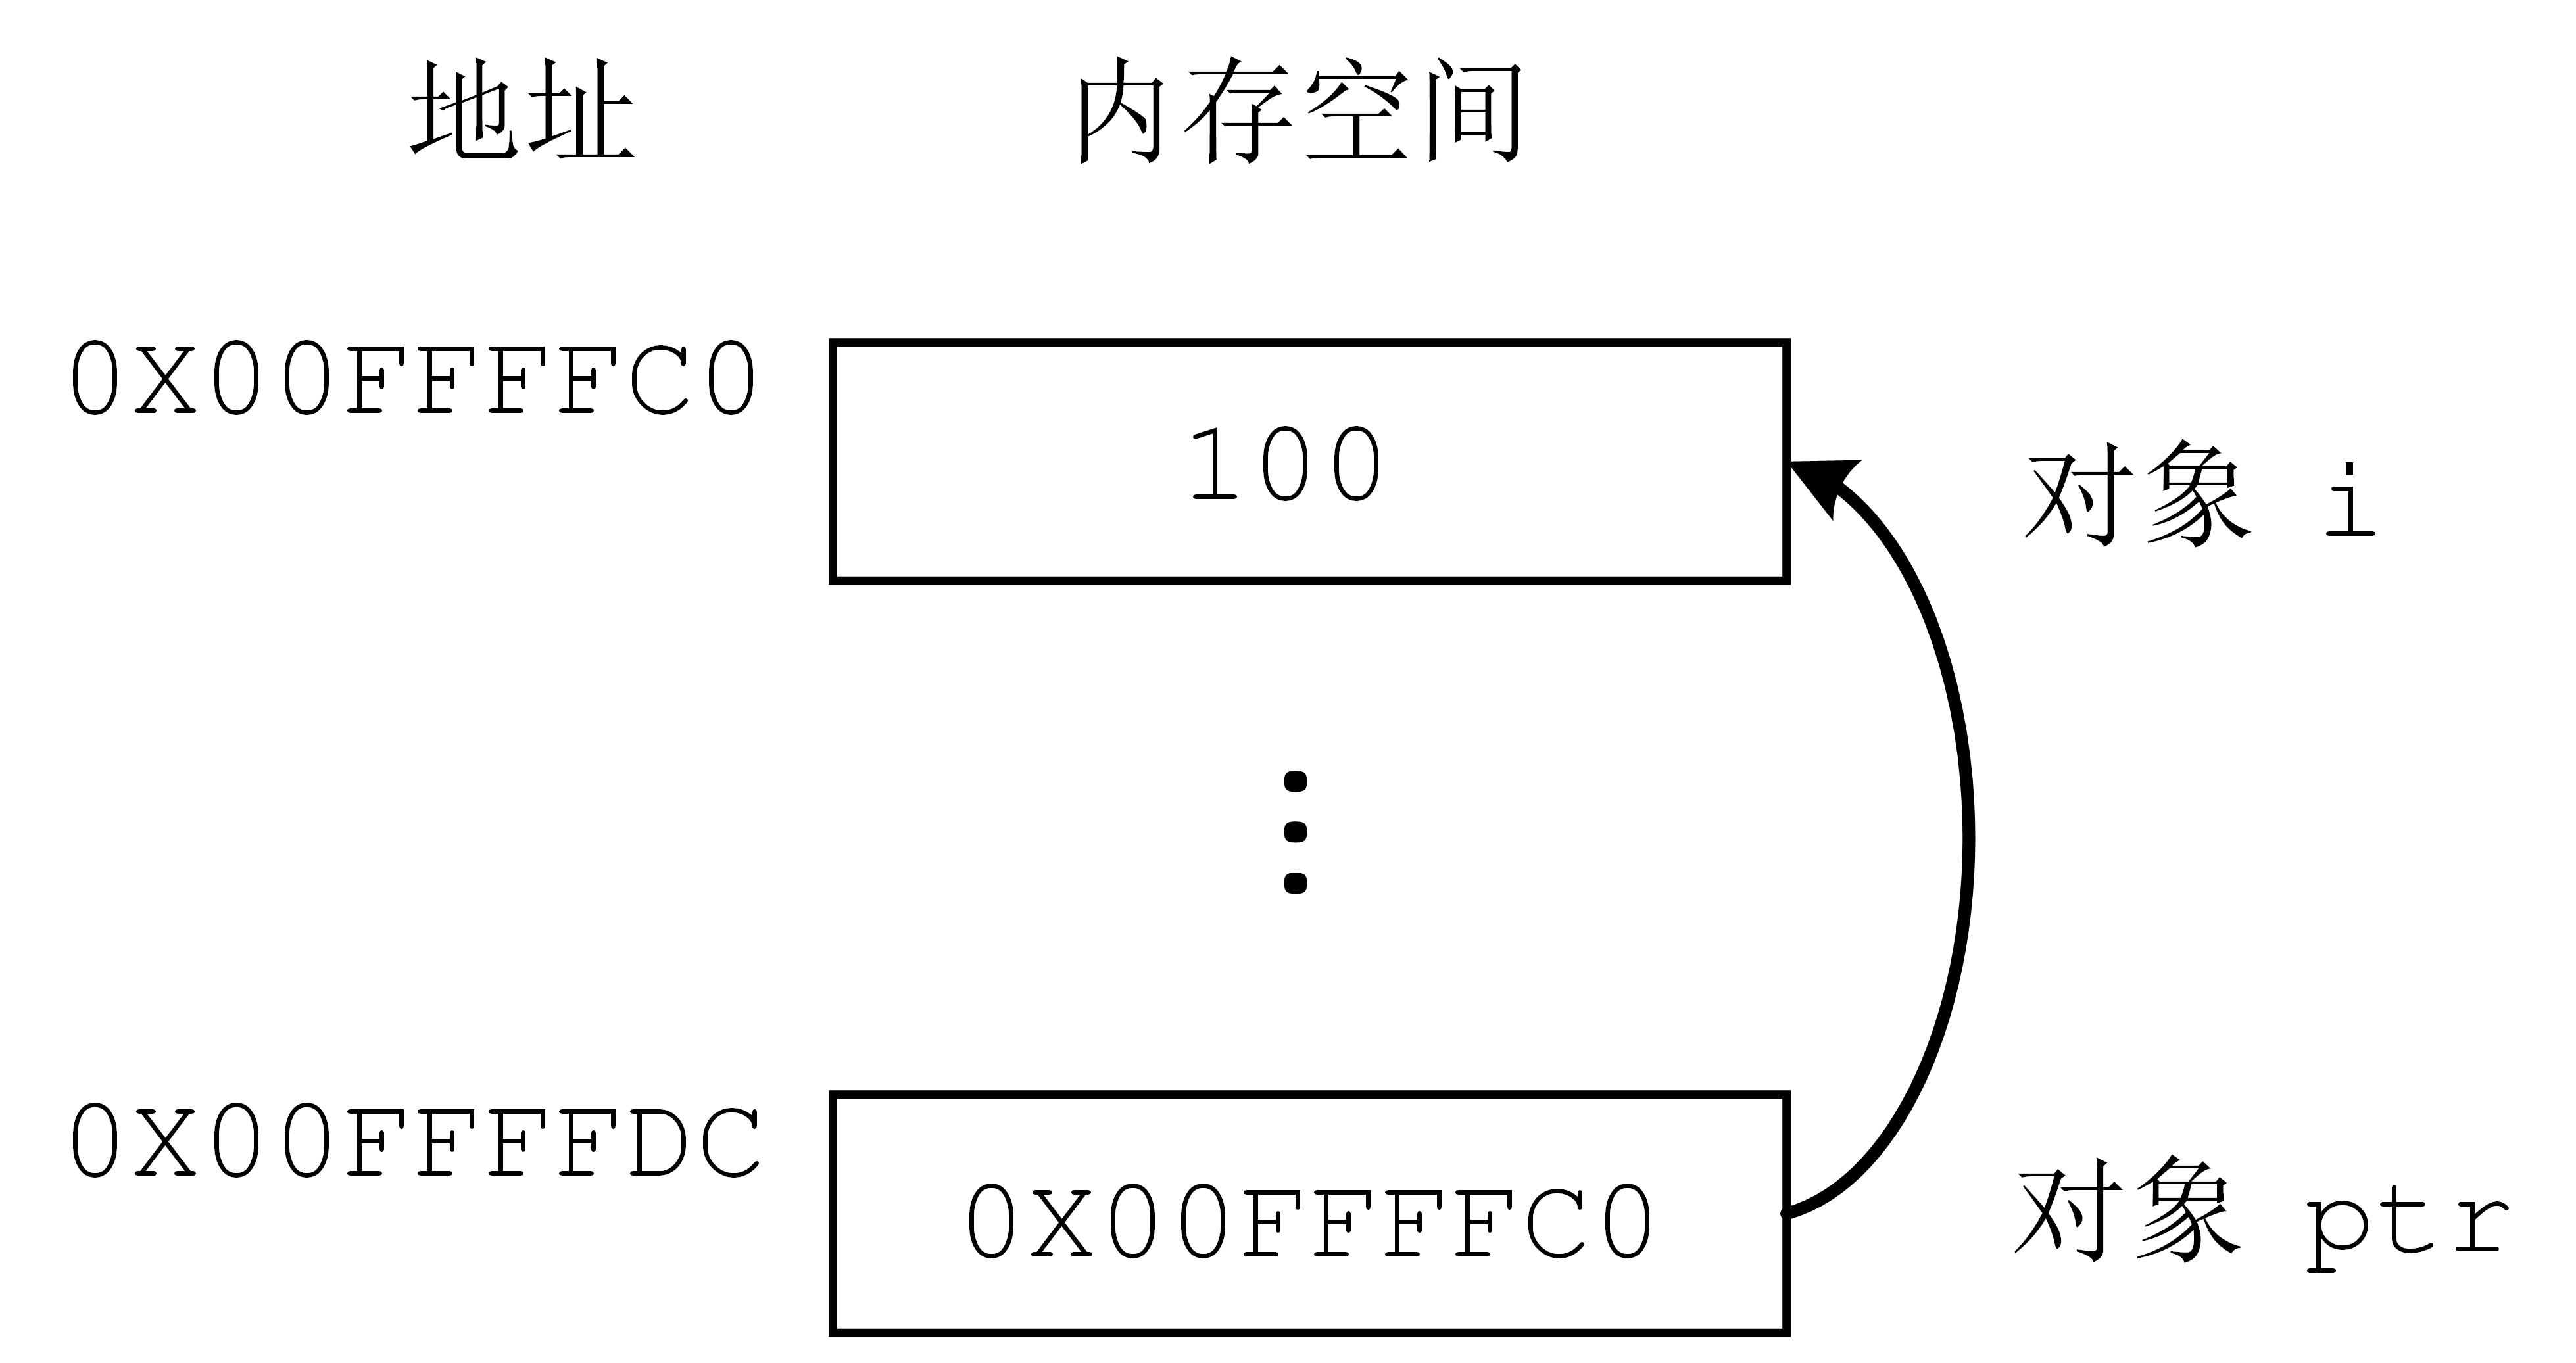
\includegraphics[scale=0.55]{Fig4-1.jpg}
		\end{column}
	\end{columns}
\end{frame}

\begin{frame}[fragile]
	\frametitle{4.2 指针\small{—指针的定义}}
	% \framesubtitle{——指针的定义}
	\begin{block}{解引用操作符(\texttt{*}):}
		如果要访问指针指向对象的内容,通过解引用操作符(\alert{\texttt{*}})来实现:
		\begin{lstlisting}[basicstyle=\small\ttfamily]
cout << *ptr << endl; //读操作,读取对象i 的内容,输出100
*ptr = 10;               //写操作,修改对象i 的内容,i 的值变为10
        \end{lstlisting}
	\end{block}
	\begin{alertblock}{提示:巧读符号}
		\begin{itemize}
			\item \texttt{*}或\texttt{\&}紧跟类型说明,为指针或引用
			\item \texttt{*}或\texttt{\&}出现在表达式中,为解引用或取址符\\
			      \ttfamily 例如:
			      \begin{lstlisting}[basicstyle=\small\ttfamily]
int i = 0;
int *ptr = &i;     //* 紧随int,故ptr 为指针;& 在表达式中,故为取址符
int &ref = *ptr;//& 紧随int,故ref 为引用;* 在表达式中,故为解引用
        \end{lstlisting}
		\end{itemize}
	\end{alertblock}
\end{frame}

\begin{frame}[fragile]
	\frametitle{4.2 指针\small{—指针的定义}}
	% \framesubtitle{——指针的定义}
	\begin{block}{定义指针对象需注意:}
		\begin{itemize}
			\item 指针的类型必须和所指向的对象的类型一致
			      \begin{lstlisting}[basicstyle=\small\ttfamily]
int i = 10;
double *ptr = &i;        //错误:ptr 和i 的类型不匹配
            \end{lstlisting}
			\item 定义多个相同类型的指针对象,每个对象名前面都要加\alert{*}
			      \begin{lstlisting}[basicstyle=\small\ttfamily]
int i, *ptr1, *ptr2; //i 为int 类型,ptr1 和ptr2 为指针对象
            \end{lstlisting}
			\item 无具体的指向对象时,需用\alert{\texttt{nullptr}}来初始化
			      \begin{lstlisting}[basicstyle=\small\ttfamily]
{
    int *ptr1 = nullptr; //ptr1 为空指针,没有指向任何对象
    int *ptr2;              //ptr2 为野指针,有潜在危险
}
            \end{lstlisting}
		\end{itemize}
	\end{block}
\end{frame}

\begin{frame}[fragile]
	\frametitle{4.2 指针\small{—改变指向}}
	% \framesubtitle{——改变指向}
	\begin{block}{改变指针指向}
		\begin{lstlisting}[basicstyle=\small\ttfamily]
int i = 10, j = 100;
int *ptr1 = &i, *ptr2 = &j; //ptr1 指向i,ptr2 指向j
ptr1 = ptr2;                 //改变ptr1 的指向,使其指向j,与ptr1 = &j 等价
ptr1 = nullptr;              //改变ptr1 的指向,ptr1 变成空指针
        \end{lstlisting}
	\end{block}
\end{frame}

\subsection{const和指针}
\begin{frame}[fragile]
	\frametitle{4.2 指针\small{—\texttt{const}和指针}}
	% \framesubtitle{——\texttt{const}和指针}
	\begin{block}{\texttt{const}和指针}
		\begin{itemize}
			\item 可以用\texttt{const}修饰符,使其不能修改所指向对象的值,即\alert{指向const对象}的指针。
			      例如:\\
			      \begin{lstlisting}[basicstyle=\small\ttfamily]
const int ci = 10, cj = 1;
const int *ptrc = &ci; //ptrc 指向常量ci
        \end{lstlisting}
		\end{itemize}
	\end{block}
	\begin{exampleblock}{练习:}
		\ttfamily 下面语句有错误吗?若有,则错在哪里?
		\begin{columns}
			\begin{column}{0.4\linewidth}
				\begin{lstlisting}[basicstyle=\small\ttfamily]
    const int a = 30;
    const int *c = &a;
    *c = 100;

    \end{lstlisting}
			\end{column}
			\hfill
			\begin{column}{0.55\linewidth}
				\onslide<2->{答案:语句\texttt{*c = 100;}错误, 不能修改所指向对象的值}
			\end{column}
		\end{columns}
	\end{exampleblock}
\end{frame}

\begin{frame}[fragile]
	\frametitle{4.2 指针\small{—\texttt{const}和指针}}
	% \framesubtitle{——\texttt{const}和指针}
	\begin{block}{\texttt{const}和指针}
		\begin{itemize}
			\item \texttt{const}修饰符修饰的指针对象,\alert{可以改变指向},甚至指向非\texttt{const}对象。\\
			      \begin{lstlisting}[basicstyle=\small\ttfamily]
const int ci = 10, cj = 1;
const int *ptrc = &ci; //ptrc 指向常量ci
ptrc = &cj;               //指向另外一个常量
int i = 0;
ptrc = &i;                //还可以指向一个非const 对象
        \end{lstlisting}
		\end{itemize}
	\end{block}
\end{frame}

\begin{frame}[fragile]
	\frametitle{4.2 指针\small{—\texttt{const}和指针}}
	% \framesubtitle{——\texttt{const}和指针}
	\begin{exampleblock}{练习:}
		\ttfamily 下面语句有错误吗?若有,则错在哪里?
		\begin{columns}
			\begin{column}{0.4\linewidth}
				\begin{lstlisting}[basicstyle=\small\ttfamily]
    const int a = 30;
    const int *c = &a;
    int b = 0;
    c = &b;
    *c = 100;
    \end{lstlisting}
			\end{column}
			\hfill
			\begin{column}{0.55\linewidth}
				\onslide<2->{答案:语句\texttt{*c = 100;}错误, 可以指向非\texttt{const}对象,但依然不能修改所指向对象的值}
			\end{column}
		\end{columns}
	\end{exampleblock}
\end{frame}

\begin{frame}[fragile]
	\frametitle{4.2 指针\small{—\texttt{const}和指针}}
	% \framesubtitle{——\texttt{const}和指针}
	\begin{block}{\texttt{const}和指针}
		\begin{itemize}
			\item 一个普通指针,不能指向\texttt{const}对象
			      \begin{lstlisting}[basicstyle=\small\ttfamily]
const int ci = 10, cj = 1;
int *ptr = &ci; //错误:ptr 不能指向常量
        \end{lstlisting}
		\end{itemize}
	\end{block}
\end{frame}

\begin{frame}[fragile]
	\frametitle{4.2 指针\small{—\texttt{const}和指针}}
	% \framesubtitle{——\texttt{const}和指针}
	\begin{block}{\texttt{const}指针}
		不允许改变指向的指针,语法格式:
		\begin{lstlisting}[basicstyle=\small\ttfamily]
int j = 0, i = 0;
int *const cptr = &i; //定义时初始化,cptr 只能指向对象i
cptr = &j;               //错误:不能改变cptr 的指向
*cptr = 10;              //正确:可以通过*cptr 修改其指向的对象i 的值
        \end{lstlisting}
	\end{block}
\end{frame}

\begin{frame}[fragile]
	\frametitle{4.2 指针\small{—\texttt{const}和指针}}
	% \framesubtitle{——\texttt{const}和指针}
	\ttfamily
	\begin{block}{指向\texttt{const}对象的\texttt{const}指针}
		\begin{lstlisting}[basicstyle=\small\ttfamily]
const int *const cptrc = &ci;//cptrc 是一个指向常量ci 的常量指针
    \end{lstlisting}
		\ttfamily 第一个~const~修饰符表明~cptrc~为一个指向~const~对象的指针,第二个~const~修饰符表明~cptrc~不能改变指向
	\end{block}
\end{frame}
\subsection{指针和类型推导}
\begin{frame}[fragile]
	\frametitle{4.2 指针\small{—类型推导和指针}}
	% \framesubtitle{——类型推导和指针}
	\begin{block}{\texttt{auto}可自动推导出指针类型}
		如果表达式的值是地址值,\texttt{auto}可以自动推导出指针类型:
		\begin{lstlisting}[basicstyle=\small\ttfamily]
int i = 0;
const int ci=10;
auto p = &i;     //p 被推导为int * 类型
auto pc = &ci;//pc 被推导为const int * 类型,ci 的const 属性被保留
        \end{lstlisting}
	\end{block}
\end{frame}

\begin{frame}[fragile]
	\frametitle{4.2 指针\small{—类型推导和指针}}
	% \framesubtitle{——类型推导和指针}
	\begin{alertblock}{提示:}
		\begin{itemize}
			\item 符号\textcolor[rgb]{1,0,0}{\texttt{\&}}和\alert{\texttt{*}}从属于对象名,并不是类型名的一部分,\texttt{auto}~只是一个“占位符”
			\item 同一条语句中定义多个对象时,对象类型必须一致,例如:\\
			      \ttfamily
			      \begin{lstlisting}[basicstyle=\small\ttfamily]
int i(0);
auto &ref = i, *ptr = &i;     //auto 被推导为int
auto &ref2 = i, ptr2 = &i; //错误:auto 的推导类型不一致
// ref2: auto被推导为int;
// ptr2: auto被推导为 int *
        \end{lstlisting}
		\end{itemize}
	\end{alertblock}
\end{frame}

\begin{frame}[fragile]
	\frametitle{4.2 指针\small{—类型推导和指针}}
	% \framesubtitle{——类型推导和指针}
	\begin{exampleblock}{练习:}
		\ttfamily 以下程序的输出结果为?
		\begin{lstlisting}[basicstyle=\small\ttfamily]
int m = 1, n = 2, *p = &m, *r;
auto q = &n;
r = p;
p = q;
q = r;
cout << m << "," << n << "," << *p << "," << *q << endl;
        \end{lstlisting}
		\onslide<2->{答案:1,2,2,1}
	\end{exampleblock}
\end{frame}

\begin{frame}[fragile]
	\frametitle{4.2 指针\small{—类型推导和指针}}
	% \framesubtitle{——类型推导和指针}
	\begin{block}{利用\texttt{decltype}进行指针类型推导}
		\begin{lstlisting}[basicstyle=\small\ttfamily]
int i = 0, *ptr = &i;
decltype (ptr) ptr2;         //ptr2 为int *
decltype (*ptr) refi = i;//正确:refi 为int &,必须初始化
decltype (*ptr+0) j;         //正确:j 为int 类型
        \end{lstlisting}
	\end{block}
\end{frame}

\begin{frame}[fragile]
	\frametitle{4.2 指针\small{—\texttt{void}指针}}
	% \framesubtitle{——\texttt{void}指针}
	\begin{block}{\texttt{void}指针}
		\begin{itemize}
			\item 能够指向任何类型的对象\\
			      \begin{lstlisting}[basicstyle=\small\ttfamily]
double x = 0;
int i = 0;
void *p = &x; //正确:可以存放double 类型对象的地址
p = &i;         //正确:也可以存放int 类型对象的地址
\end{lstlisting}
		\end{itemize}
	\end{block}
	\begin{alertblock}{提示:}
		将\texttt{void}指针赋值给普通指针,必须确保它们指向的对象类型相同,需要进行类型转换\\
		\ttfamily
		例如:\\
		\begin{lstlisting}[basicstyle=\small\ttfamily]
double x = 0, *ptrd = &x;
void *ptr = &x;
ptrd = ptr; //报错:不能直接将void指针赋值double *类型的指针。正确语句:
ptrd = static_cast<double *>(ptr);
        \end{lstlisting}
	\end{alertblock}
\end{frame}

\begin{frame}[fragile]
	\frametitle{4.2 指针\small{多级指针}}
	% \framesubtitle{——多级指针}
	\begin{block}{二级指针}
		将一个指针对象的地址存放到另一个指针对象中即构成\alert{多级指针}(二级指针)。格式如下:\\
		\begin{lstlisting}[basicstyle=\small\ttfamily]
int i = 1, *ptr = &i;
int **pptr = &ptr; //用指针对象ptr 的地址初始化pptr
        \end{lstlisting}
		可用三种方式访问对象\texttt{i}:\\
		\begin{lstlisting}[basicstyle=\small\ttfamily]
cout << i << '\t' << *ptr << '\t' << **pptr << endl;
        \end{lstlisting}
	\end{block}
	\begin{block}{三级指针}
		\begin{lstlisting}[basicstyle=\small\ttfamily]
int ***ppptr = &pptr;
cout << ***ppptr << endl; //输出1
        \end{lstlisting}
	\end{block}
\end{frame}
\subsection{指针和引用}
\begin{frame}[fragile]
	\frametitle{4.2 指针\small{—引用和指针}}
	% \framesubtitle{——引用和指针}
	\begin{block}{引用和指针的区别:}
		\begin{itemize}
			\item 定义引用时\alert{必须初始化},定义指针时不需要初始化:\\
			      \begin{lstlisting}[basicstyle=\small\ttfamily]
int i = 0, j = 1;
int &r;//错误:引用在定义时需要给定初始值
int *p;//正确
            \end{lstlisting}
			\item \alert{不存在空引用}。引用必须与有效的内存单元关联,指针可以为\texttt{nullptr};
			\item \alert{赋值行为不同}。对引用赋值修改与其相绑定的对象的值,对指针赋值改变其指向的对象,例如:\\
			      \begin{lstlisting}[basicstyle=\small\ttfamily]
int i = 0, j = 1, &r = i, *p = &i;
r = 4;   //修改与r 相绑定的对象i 的值
p = &j; //修改指针p 的值,使其指向j
            \end{lstlisting}
		\end{itemize}
	\end{block}
\end{frame}

\begin{frame}[fragile]
	\frametitle{4.2 指针\small{—引用和指针}}
	% \framesubtitle{——引用和指针}
	\begin{block}{引用和指针}
		\alert{引用}的行为实际上类似于\alert{\texttt{const}指针}的行为,可以把引用看作是支持自动解引用操作的\texttt{const}指针:
		\begin{lstlisting}[basicstyle=\small\ttfamily]
int i = 0;
int *const p = &i; //不允许指针p指向其他对象
int &ri = i;          //引用 ri 只能与 i 绑定
    \end{lstlisting}
	\end{block}
	\begin{alertblock}{建议:}
		能用引用的地方,不要用指针。
	\end{alertblock}
\end{frame}

\section{数组}
\subsection{定义和初始化}
\begin{frame}[fragile]
	\frametitle{4.3 数组\small{—数组的定义和初始化}}
	% \framesubtitle{——数组的定义和初始化}
	% \ttfamily
	\begin{block}{数组---\color{yellow}{处理批量数据}}
		\alert{数组}是由有限个\alert{同类型}元素组成的\alert{有序集合},所有元素顺序存放在一段连续的内存空间中。\\如下定义一个存储5个整型元素的数组:\\
		\begin{lstlisting}[basicstyle=\small\ttfamily]
int arr[5];
        \end{lstlisting}
	\end{block}
	\begin{minipage}[m]{0.3\linewidth}
		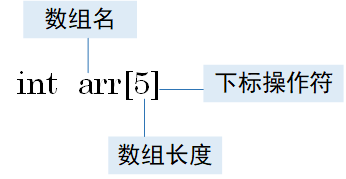
\includegraphics[scale=0.4]{array.png}
	\end{minipage}
	\hfill
	\begin{minipage}[m]{0.48\linewidth}
		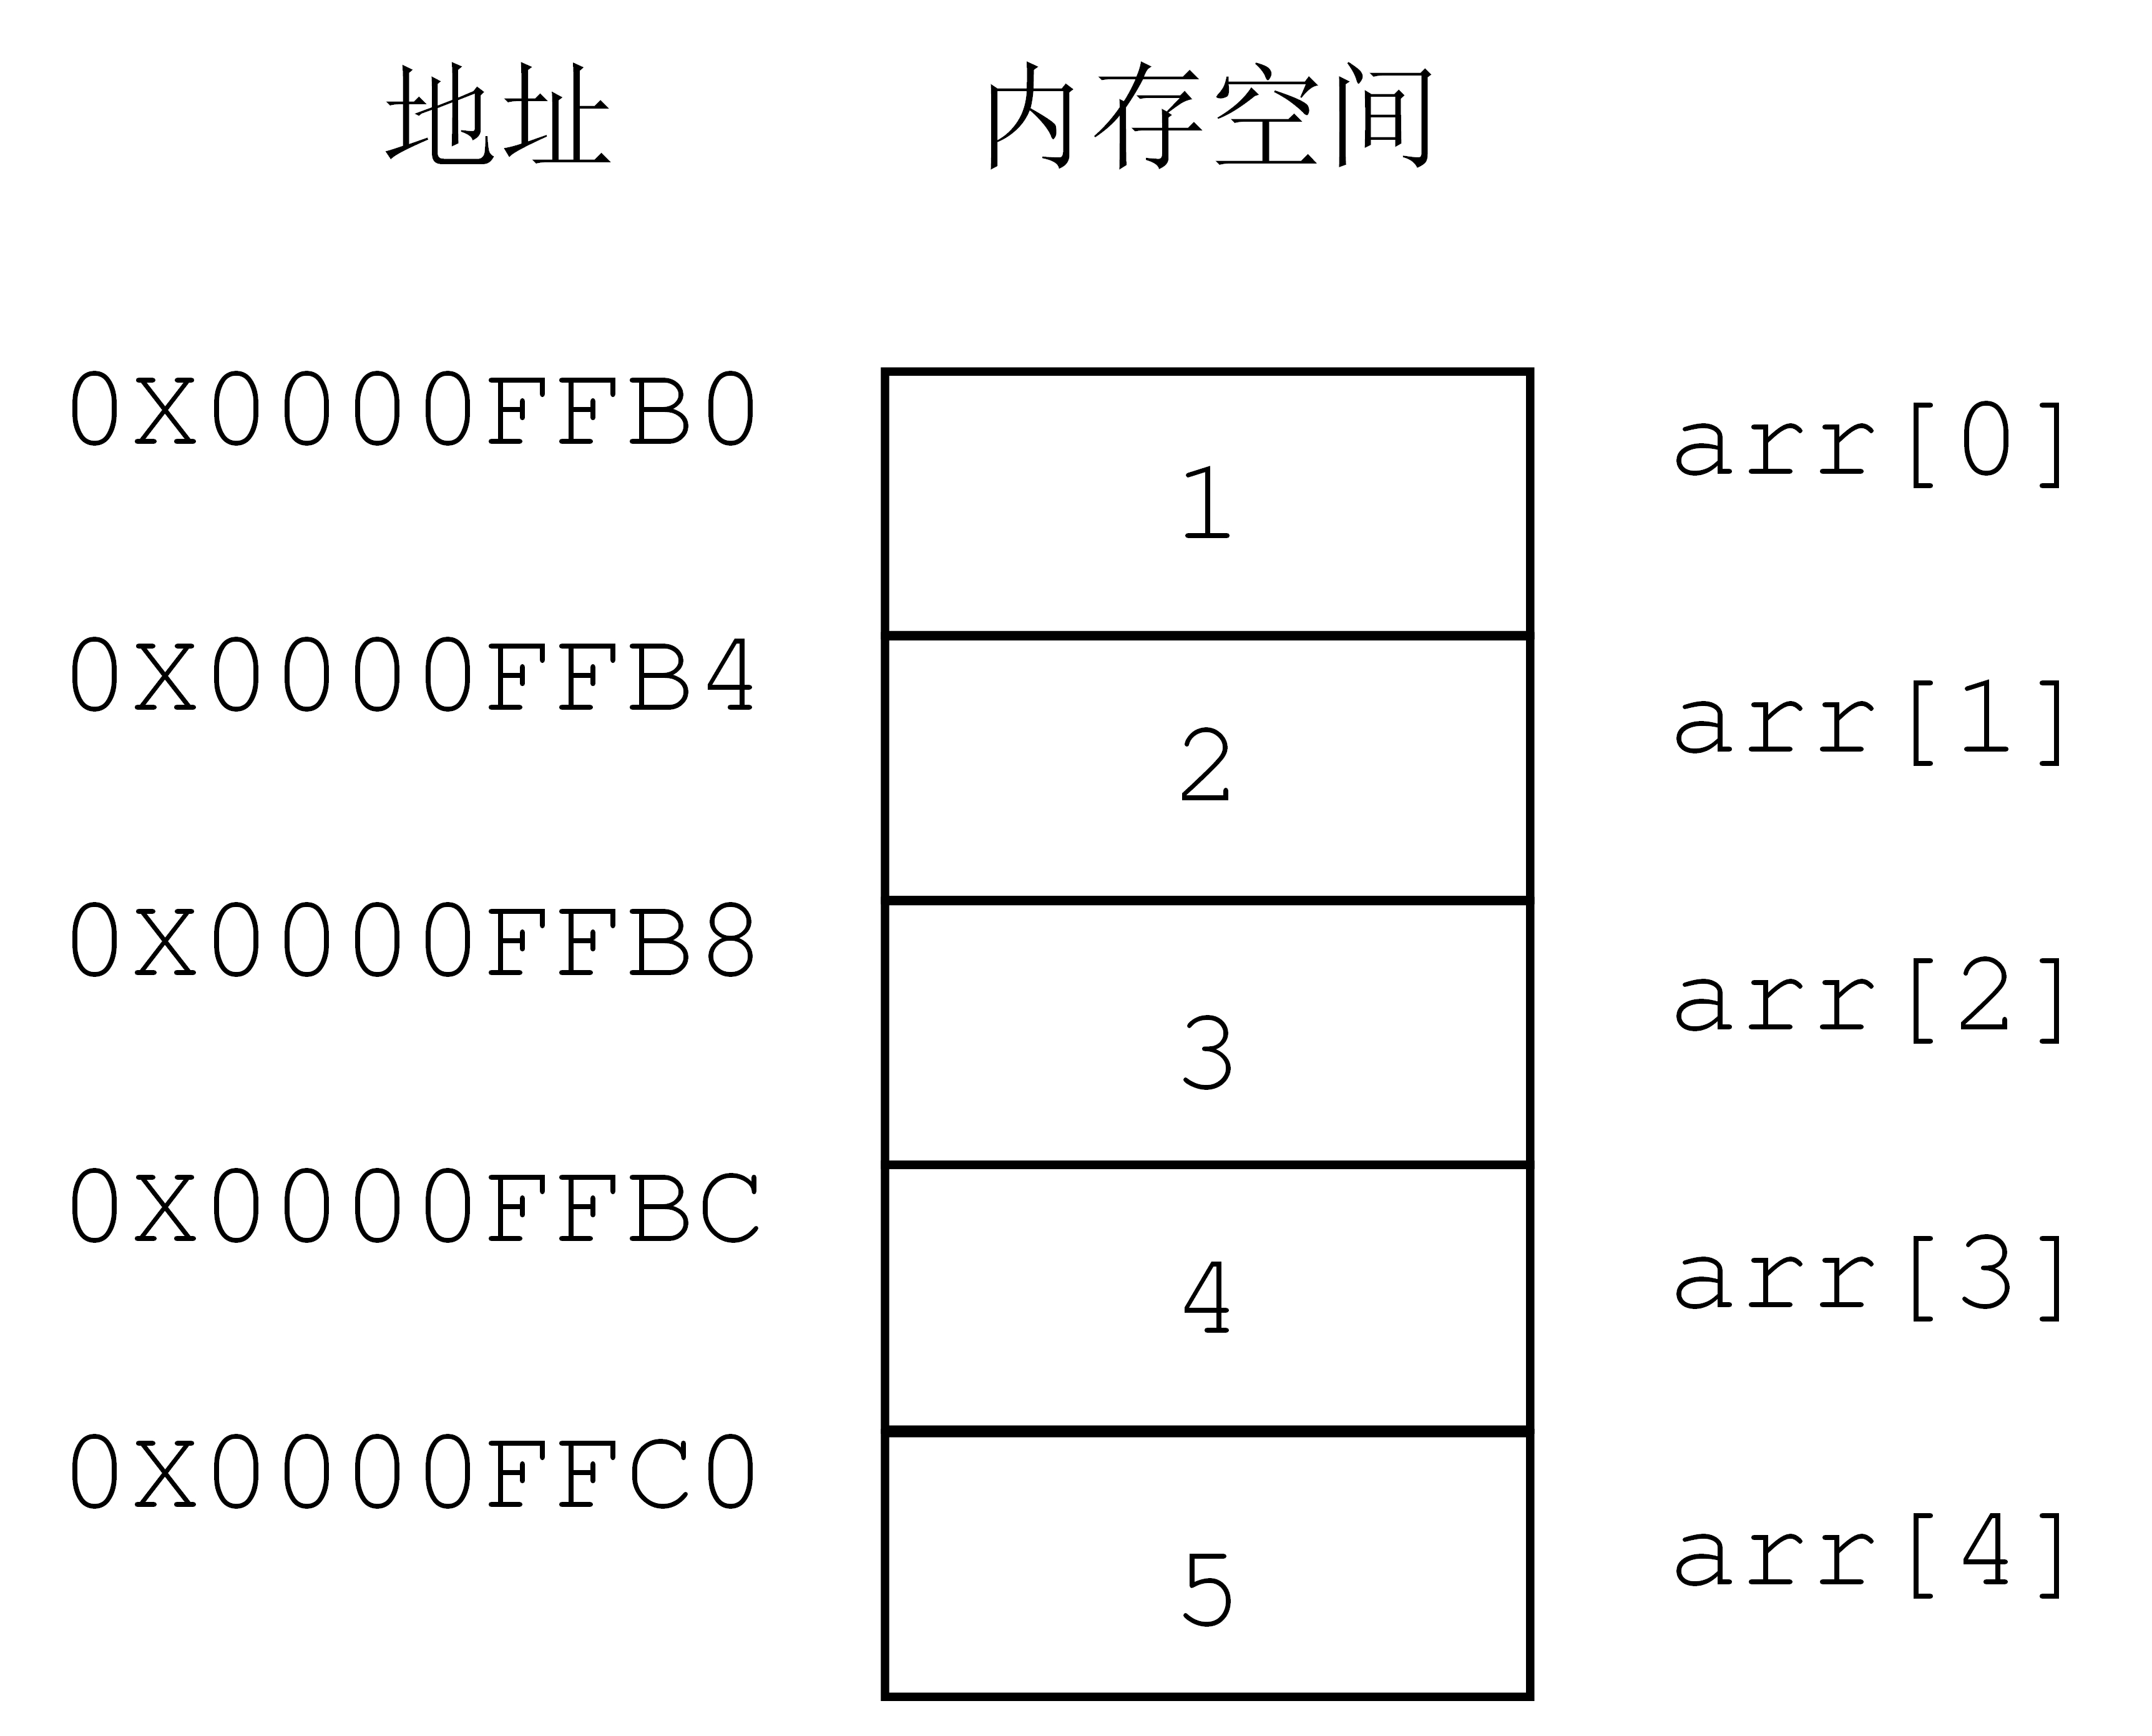
\includegraphics[scale=0.6]{Fig4-2.jpg}
	\end{minipage}
\end{frame}


\begin{frame}[fragile]
	\frametitle{4.3 数组\small{—数组的定义和初始化}}
	% \framesubtitle{——数组的定义和初始化}
	\begin{block}{数组长度}
		数组长度必须为大于0的整型常量表达式:
		\begin{lstlisting}[basicstyle=\small\ttfamily]
unsigned cnt = 10;
int arr[cnt];              //错误,cnt 不是常量表达式
constexpr int sz = 10; //常量表达式
int arri[sz];             //正确:存放10 个整型数据的数组
float arrf[10.];          //错误:数组长度必须是整型
        \end{lstlisting}
		其中,第三行代码中的\texttt{constexpr}可用\texttt{const}代替
	\end{block}
\end{frame}

\begin{frame}[fragile]
	\frametitle{4.3 数组\small{—数组的定义和初始化}}
	% \framesubtitle{——数组的定义和初始化}
	% \ttfamily
	\begin{block}{数组的初始化}
		\begin{itemize}
			\item 未显式初始化,则用默认的方式初始化。通常采用\alert{列表初始化}显式初始化数组元素:
			      \begin{lstlisting}[basicstyle=\small\ttfamily]
int arr[5] = {1, 2, 3, 4, 5};
            \end{lstlisting}
			\item 显式初始化部分数组元素:
			      \begin{lstlisting}[basicstyle=\small\ttfamily]
int arr[5] = {1, 2, 3}; //等价于arr[5] = {1, 2, 3, 0, 0}
            \end{lstlisting}
			\item 编译器可以根据列表中提供的元素的个数,推断数组的长度:
			      \begin{lstlisting}[basicstyle=\small\ttfamily]
int arr[] = {1, 2, 3, 4, 5}; //数组arr 的长度为5
            \end{lstlisting}
		\end{itemize}
	\end{block}
\end{frame}

\begin{frame}[fragile]
	\frametitle{4.3 数组\small{—数组的定义和初始化}}
	% \framesubtitle{——数组的定义和初始化}
	% \ttfamily
	\begin{block}{字符数组}
		\begin{itemize}
			\item 采用\alert{字符串字面值}来初始化,例如:
			      \begin{lstlisting}[basicstyle=\small\ttfamily]
char name[] = "Lisha"; //自动添加字符串结束符'\0'
            \end{lstlisting}
			\item 这种方式等价于:
			      \begin{lstlisting}[basicstyle=\small\ttfamily]
char name[] = {'L', 'i', 's', 'h', 'a', '\0'};
            \end{lstlisting}
		\end{itemize}
	\end{block}
	\begin{alertblock}{提示:}
		上面的语句是\alert{初始化操作},\alert{不是赋值操作}。不能将字符串常量赋值给一个数组,如:
		\begin{lstlisting}[basicstyle=\small\ttfamily]
name = "Lisha"; //错误:数组不允许赋值操作
        \end{lstlisting}
	\end{alertblock}
\end{frame}

\begin{frame}[fragile]
	\frametitle{4.3 数组\small{—数组的定义和初始化}}
	% \framesubtitle{——数组的定义和初始化}
	\begin{alertblock}{注意:数组中的数据不能整体操作}
		不能用一个数组初始化另外一个数组,也不能用一个数组赋值给另外一个数组\\
		\begin{lstlisting}[basicstyle=\small\ttfamily]
char n1[] = "Lisha";
char n2[] = n1; //错误:不能用数组初始化数组
n2 = n1; //错误:数组不能执行赋值操作
        \end{lstlisting}
	\end{alertblock}
\end{frame}


\begin{frame}[fragile]
	\frametitle{4.3 数组\small{—数组的定义和初始化}}
	% \framesubtitle{——数组的定义和初始化}
	% \ttfamily
	\begin{block}{复杂数组的定义}
		\begin{itemize}
			\item 数组元素的类型是指针,即指针数组:
			      \begin{lstlisting}[basicstyle=\small\ttfamily]
int arr[5];     //定义一个含有5 个int 类型元素的数组
int *arrp[5]; //含有5 个int* 类型元素的数组,每个元素都是指针
        \end{lstlisting}
			\item 数组指向其他数组,即数组指针:
			      \begin{lstlisting}[basicstyle=\small\ttfamily]
int (*parr)[5] = &arr; //指向含有5 个int 类型元素的数组的指针
        \end{lstlisting}
			\item 数组引用其他数组,即数组的引用:
			      \begin{lstlisting}[basicstyle=\small\ttfamily]
int (&rarr)[5] = arr; //定义arr 的一个引用定义
        \end{lstlisting}
		\end{itemize}
	\end{block}
\end{frame}

\begin{frame}[fragile]
	\frametitle{4.3 数组\small{—数组的定义和初始化}}
	% \framesubtitle{——数组的定义和初始化}
	\begin{block}{定义一个指向\texttt{arrp}的指针或引用:}
		\ttfamily
int *arrp[5]; \\
		int *(*parrp)[5] = \&arrp;\\
		int *(\&rarrp)[5] = arrp;\\
		parrp~和~rarrp~分别为指向指针数组~arrp~的指针和引用。
	\end{block}
\end{frame}

\begin{frame}[fragile]
	\frametitle{4.3 数组\small{—访问数组元素}}
	% \framesubtitle{——访问数组元素}
	% \ttfamily
	\begin{block}{通过下标操作符\texttt{[]}访问数组元素:}
		\begin{lstlisting}[basicstyle=\small\ttfamily]
int arr[5] ={1, 2, 3, 4, 5} ;
arr[0] = 10;                //写操作:修改第一个元素的值
cout << arr[0] <<" "<< arr[4] <<endl; //读操作,输出结果为:10 5
        \end{lstlisting}
	\end{block}
	\begin{alertblock}{提示:}
		\texttt{C++}不检查下标索引值是否有效,如:
		\begin{lstlisting}[basicstyle=\small\ttfamily]
cout << arr[5] << endl; //编译器不提示错误,程序可以运行,输出为:-858993460
        \end{lstlisting}
	\end{alertblock}
\end{frame}

\begin{frame}[fragile]
	\frametitle{4.3 数组\small{—访问数组元素}}
	% \framesubtitle{——访问数组元素}
	\begin{block}{范围\texttt{for(range for)}语句}
		语法格式如下:\\
		\begin{lstlisting}[basicstyle=\small\ttfamily]
            for(decl : expr){
                statement;
            }
                \end{lstlisting}
		\begin{itemize}
			\item \texttt{expr}必须是\alert{对象序列},比如数组、容器(\texttt{vector})或字符串(\texttt{string})
			\item \texttt{decl}是与序列中数据元素类型相同的对象,通常用\texttt{auto}来推导数据元素的类型
		\end{itemize}
	\end{block}
\end{frame}

\begin{frame}[fragile]
	\frametitle{4.3 数组\small{—访问数组元素}}
	% \framesubtitle{——访问数组元素}
	\begin{exampleblock}{示例:}
		\begin{lstlisting}[basicstyle=\small\ttfamily]
int arr[5]={1,2,3,4,5};  //定义并初始化一个含有5 个整型数的数组
for(auto i: arr){           //i 为arr 中当前元素的副本
    cout << i << endl;    //打印输出当前获取的整数
}
        \end{lstlisting}
	\end{exampleblock}
	\begin{columns}
		\begin{column}{0.25\linewidth}
			
\includegraphics[scale=0.3]{quetion_icon1.png}
		\end{column}
		\hfill
		\begin{column}{0.7\linewidth}
			\begin{thinkblock}{思考:}
				上述\texttt{range for}语句可以对对象的内容进行修改吗?
		\begin{lstlisting}[basicstyle=\small\ttfamily]
for(auto i: arr){  
    i =0;    
}
        \end{lstlisting}
			\end{thinkblock}
		\end{column}
	\end{columns}
\end{frame}

\begin{frame}[fragile]
	\frametitle{4.3 数组\small{—访问数组元素}}
	% \framesubtitle{——访问数组元素}
	\begin{block}{利用\texttt{range for}对数组元素进行写操作}
		需将\texttt{decl}声明为引用
		\begin{lstlisting}[basicstyle=\small\ttfamily]
for(auto &i: arr){ //i为arr中当前元素的引用
    i = 0;            //写操作:每一个元素设置为0
}
        \end{lstlisting}
	\end{block}
\end{frame}

\begin{frame}
	\frametitle{4.3 数组\small{—访问数组元素}}
	% \framesubtitle{——访问数组元素}
	% \ttfamily
	\begin{exampleblock}{例4.1:}
		\ttfamily
		计算一个班级30名学生的数学科目的平均成绩和标准差。学生成绩随机生成。\\
		\alert{提示}:标准差公式:$\sigma=\sqrt{\frac{\sum\limits_{i=1}^{N}(X_{i}-\mu)^{2}}{N}}$
	\end{exampleblock}
	\centering
	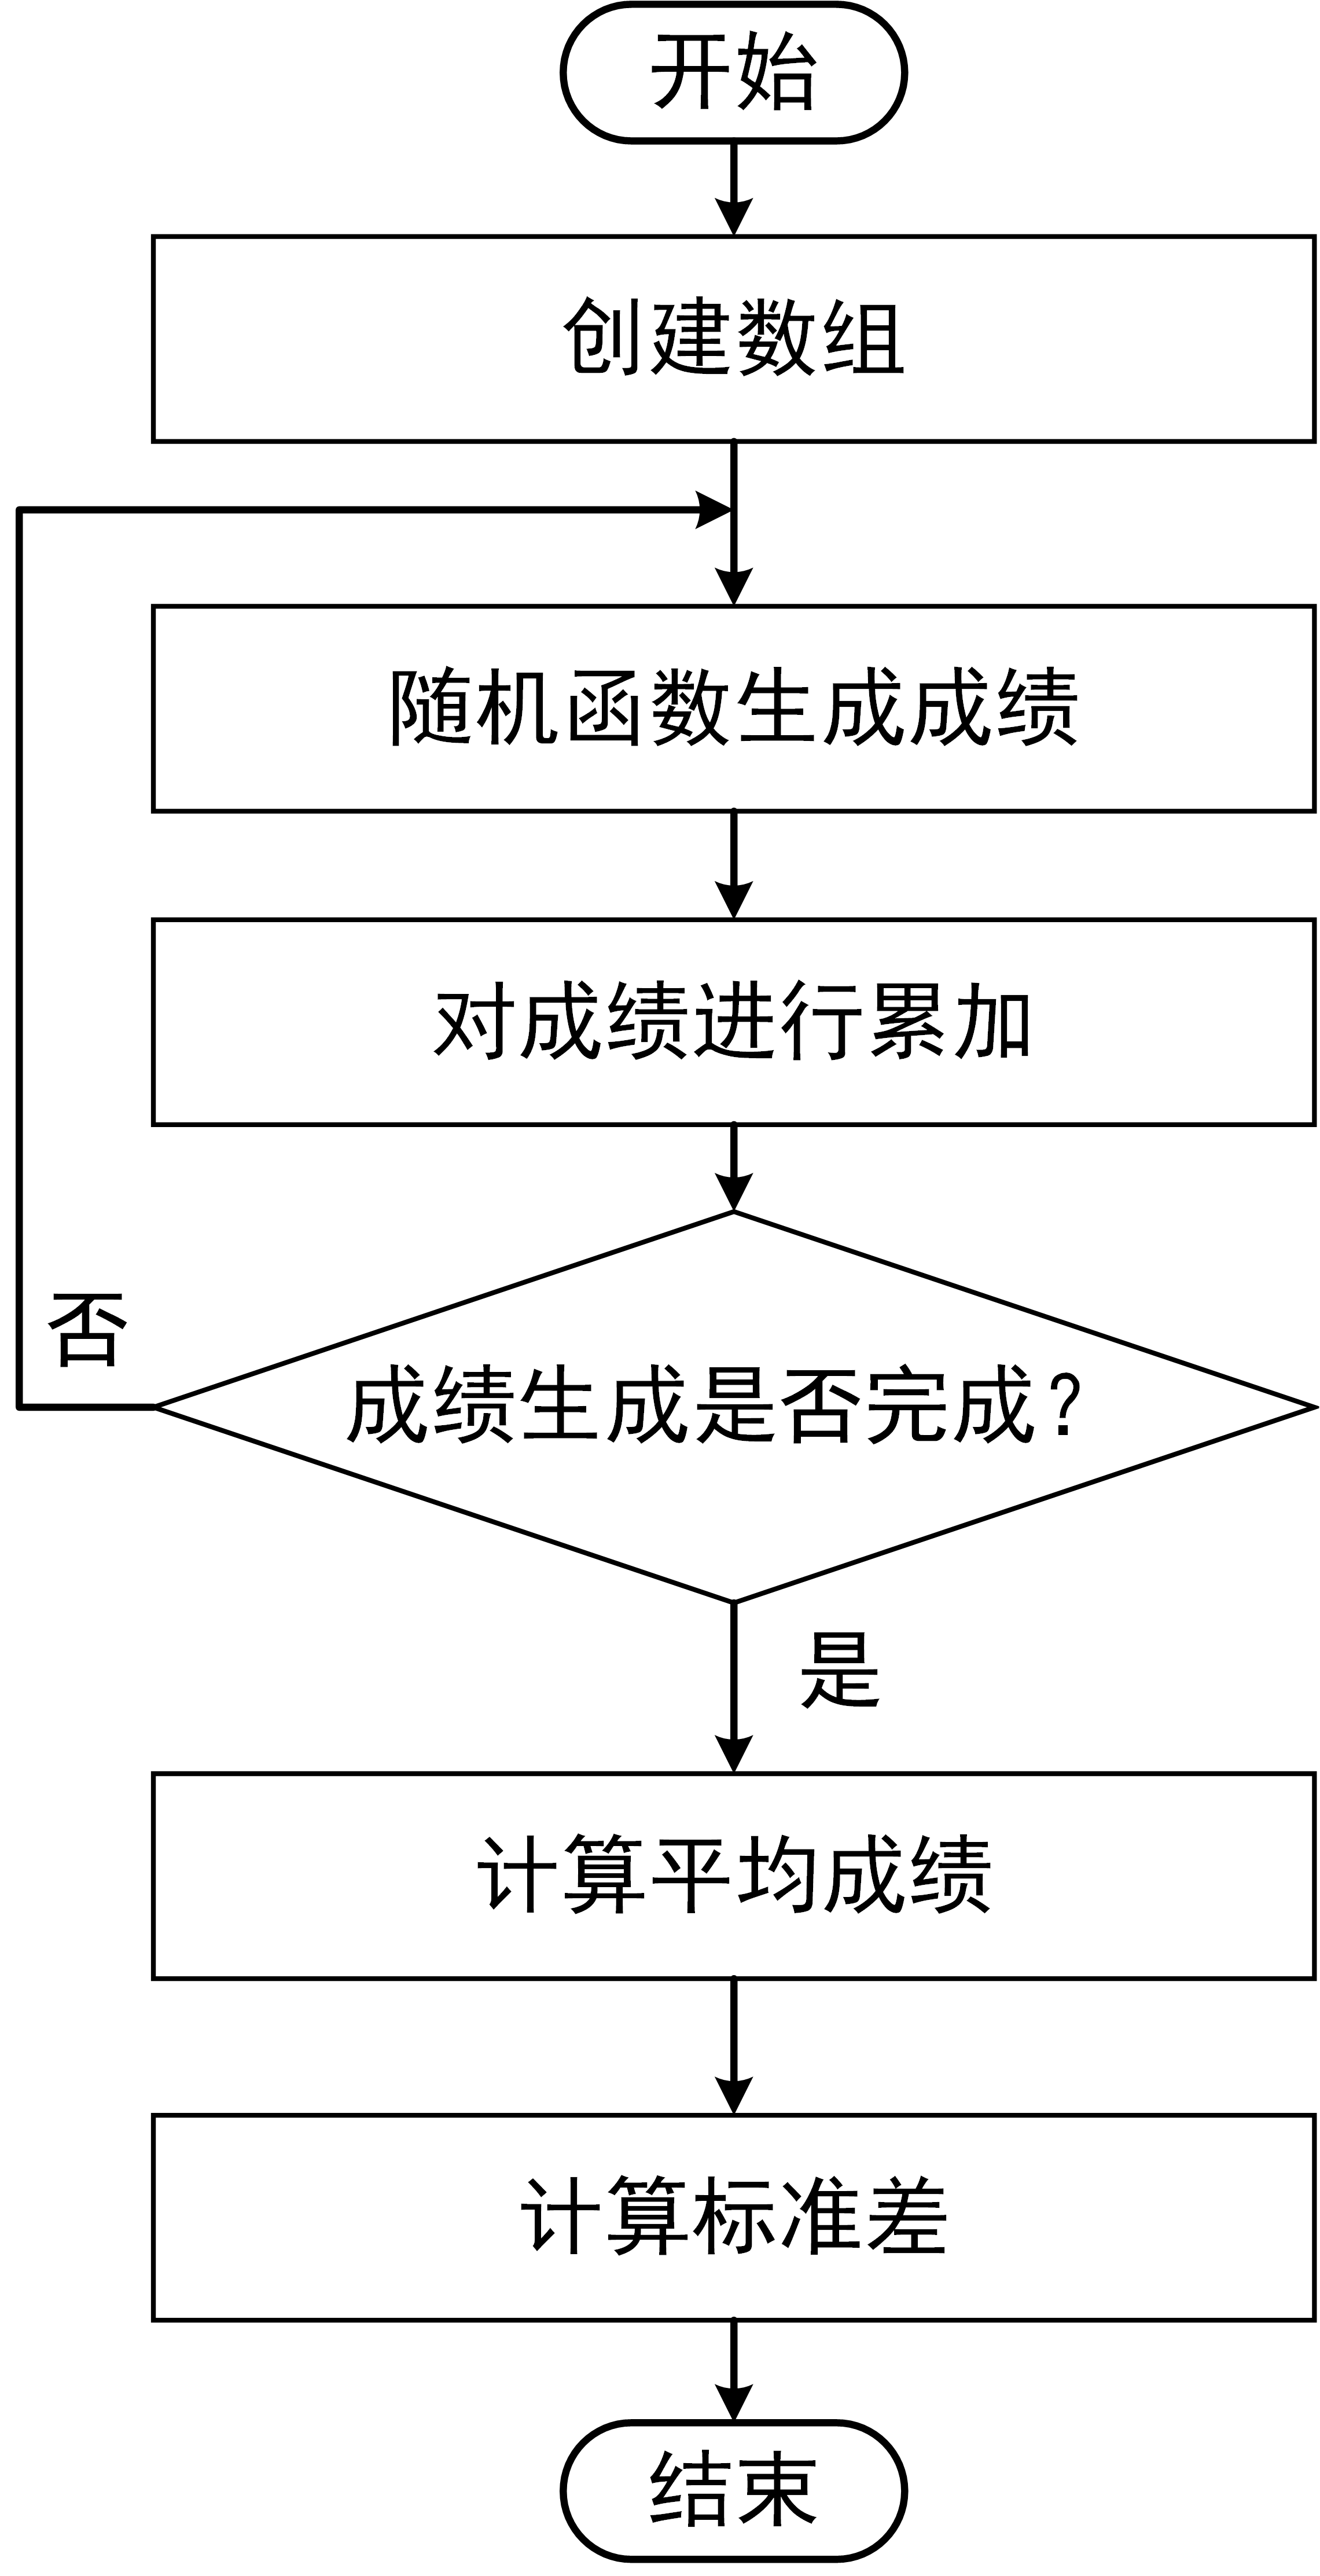
\includegraphics[scale=0.28]{example4_1.png}
\end{frame}

\begin{frame}[fragile]
	\frametitle{4.3 数组\small{—访问数组元素}}
	% \framesubtitle{——访问数组元素}
	\begin{exampleblock}{代码清单4.1,例4.1:}
		% \begin{minipage}[t]{0.4\linewidth}
		\begin{columns}
			\begin{column}{0.06\linewidth}
			\end{column}
			\begin{column}{0.94\textwidth}
				\begin{lstlisting}[numbers=left,numberstyle=\small,basicstyle=\small\ttfamily]
#include <cstdlib>
#include <iostream>
using namespace std;
int main() {
    srand(0);//使用固定种子,每次运行得到一样的结果,有助于调式
    constexpr int sz = 30;
    int score[sz]; //定义一个数组,存放30个学生的成绩
    int mean = 0;//存放平均分数, 初始值必须为0
    for (auto &i:score) //使用范围for语句访问,注意引用&不能丢
        i = 50 + rand() % 51;//成绩随机分布在50到100之间
        mean += i;//累加每一个学生成绩到mean里面
    }
    mean /= sz;//计算平均成绩
        \end{lstlisting}\ttfamily
			\end{column}
		\end{columns}
	\end{exampleblock}
\end{frame}

\begin{frame}[fragile]
	\frametitle{4.3 数组\small{—访问数组元素}}
	% \framesubtitle{——访问数组元素}
	\begin{exampleblock}{代码清单4.1,例4.1:}
		% \begin{minipage}[t]{0.4\linewidth}
		\begin{columns}
			\begin{column}{0.06\linewidth}
			\end{column}
			\begin{column}{0.94\textwidth}
				\begin{lstlisting}[numbers=left,numberstyle=\small,firstnumber=14,basicstyle=\small\ttfamily]
    double dev = 0;
    for (int i = 0; i < sz; ++i)
        dev += pow(score[i]- mean,2);//函数pow(x,a)计算x^a
    }
    dev = sqrt(dev / sz);
    cout << "平均成绩:" << mean <<" 标准差:"<< dev << endl;
    return 0;
}
        \end{lstlisting}
			\end{column}
		\end{columns}
	\end{exampleblock}
\end{frame}

\begin{frame}
	\frametitle{4.3 数组\small{—访问数组元素}}
	% \framesubtitle{——访问数组元素}
	% \ttfamily
	\begin{exampleblock}{例4.2:}
		\ttfamily
		在8$\times$8的国际象棋棋盘上摆放八个皇后,使其不能相互攻击,即任意两个皇后不得处在同一行、同一列或者同一对角斜线上。下图所示是一种符合条件的摆放方案。本题计算出一种方案即可。\\
		\alert{提示}:用回溯法求解。回溯法基本思想:当探索到某一步时,发现原先选择并不优或达不到目标,就退回一步重新选择,即走不通就退回重新走。
	\end{exampleblock}
	% 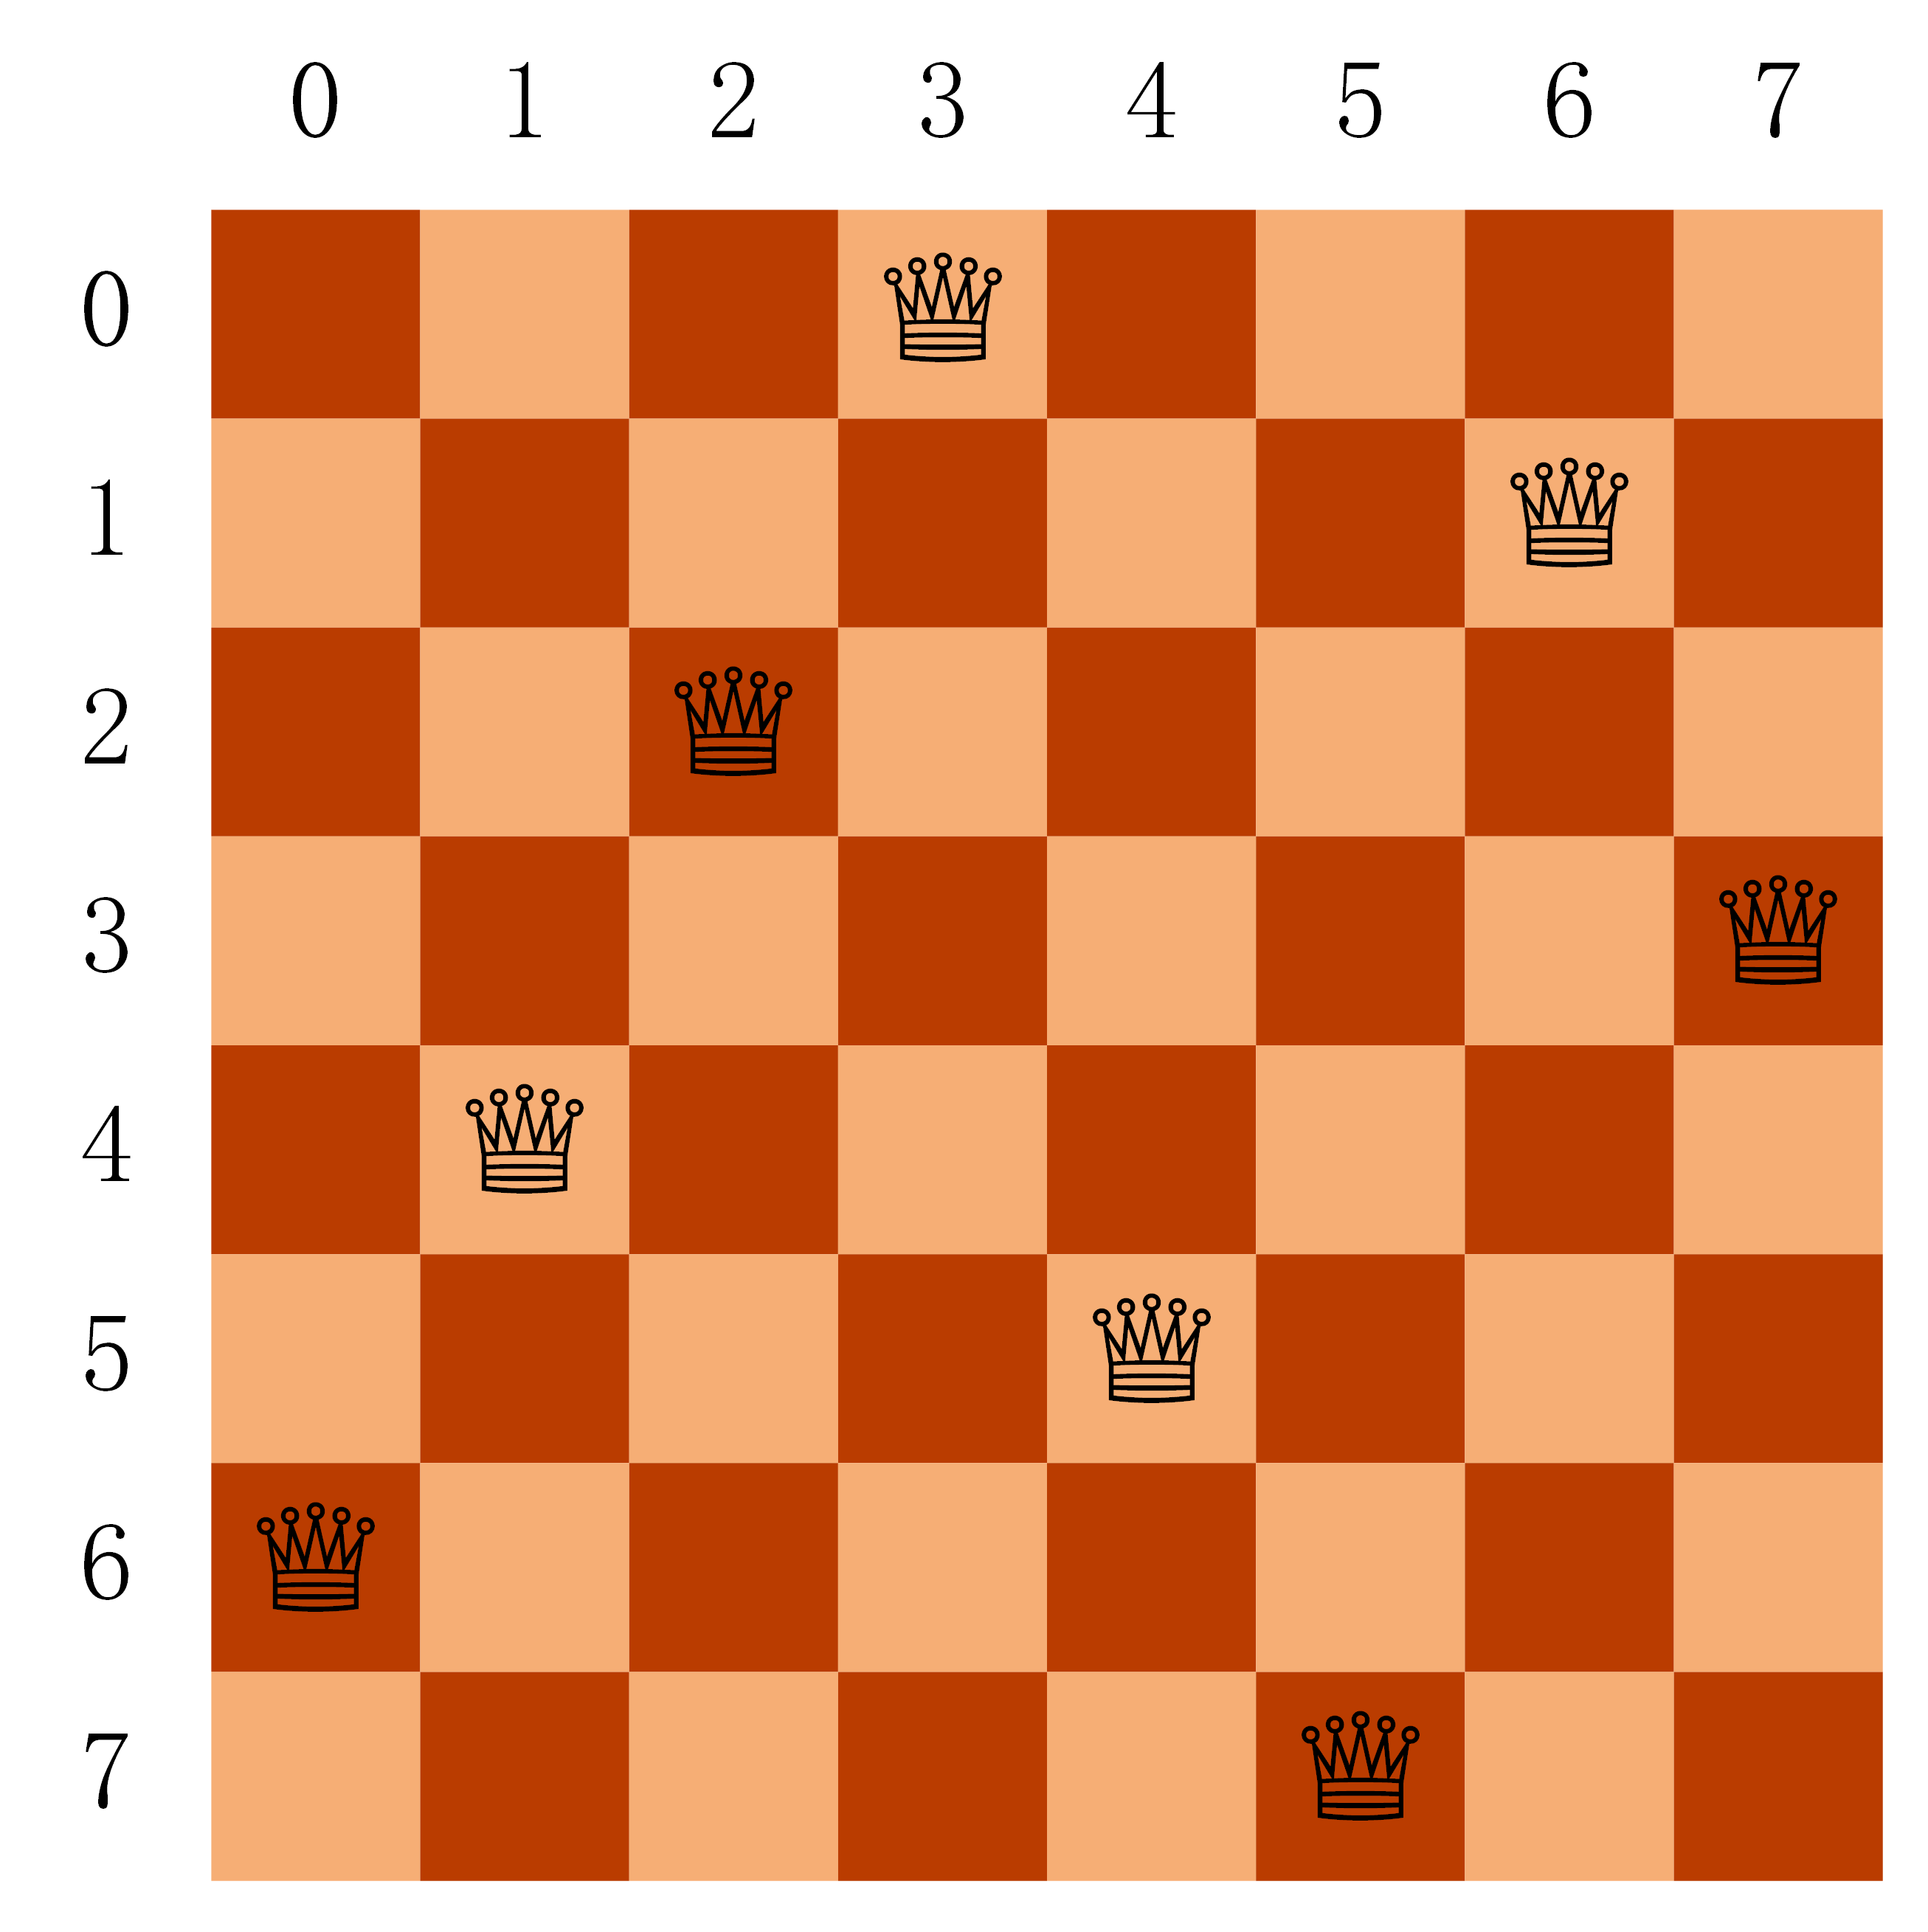
\includegraphics[scale=0.35]{Fig4-3.png}
	\begin{figure}
		\centering
		\animategraphics[scale=1.3,autoplay]{2}{example4_2/example4_2_}{001}{114}
	\end{figure}
\end{frame}

\begin{frame}
	\frametitle{4.3 数组\small{—访问数组元素}}
\begin{columns}
    \begin{column}{0.6\linewidth}
        \begin{exampleblock}{例4.2:解的表示}
        		\ttfamily
        		用一个数组~que[8]~来存放每一个皇后的位置,如~que[0]=3~代表第0行的皇后在第3列。\\
        ~~~~que[8] = \{3, 6, 2, 7, 1, 4, 0, 5\};\\
        ~~~~\\
        冲突情况:\\
        1)第~i~行和第~j~行的皇后在同一列:\\
        ~~~~ que[i] == que[j]\\
        2)第~i~行和第~j~行的皇后在同一对角线上:\\
        ~~~~ {|que[i] - que[j]| == |i - j|}\\
        比如~que[0]=1,que[1]=2~表明第0行和第1行的两个皇后在同一个对角线上。
        \end{exampleblock}
    \end{column}
	\begin{column}{0.4\textwidth}
        \begin{figure}
        \centering
        	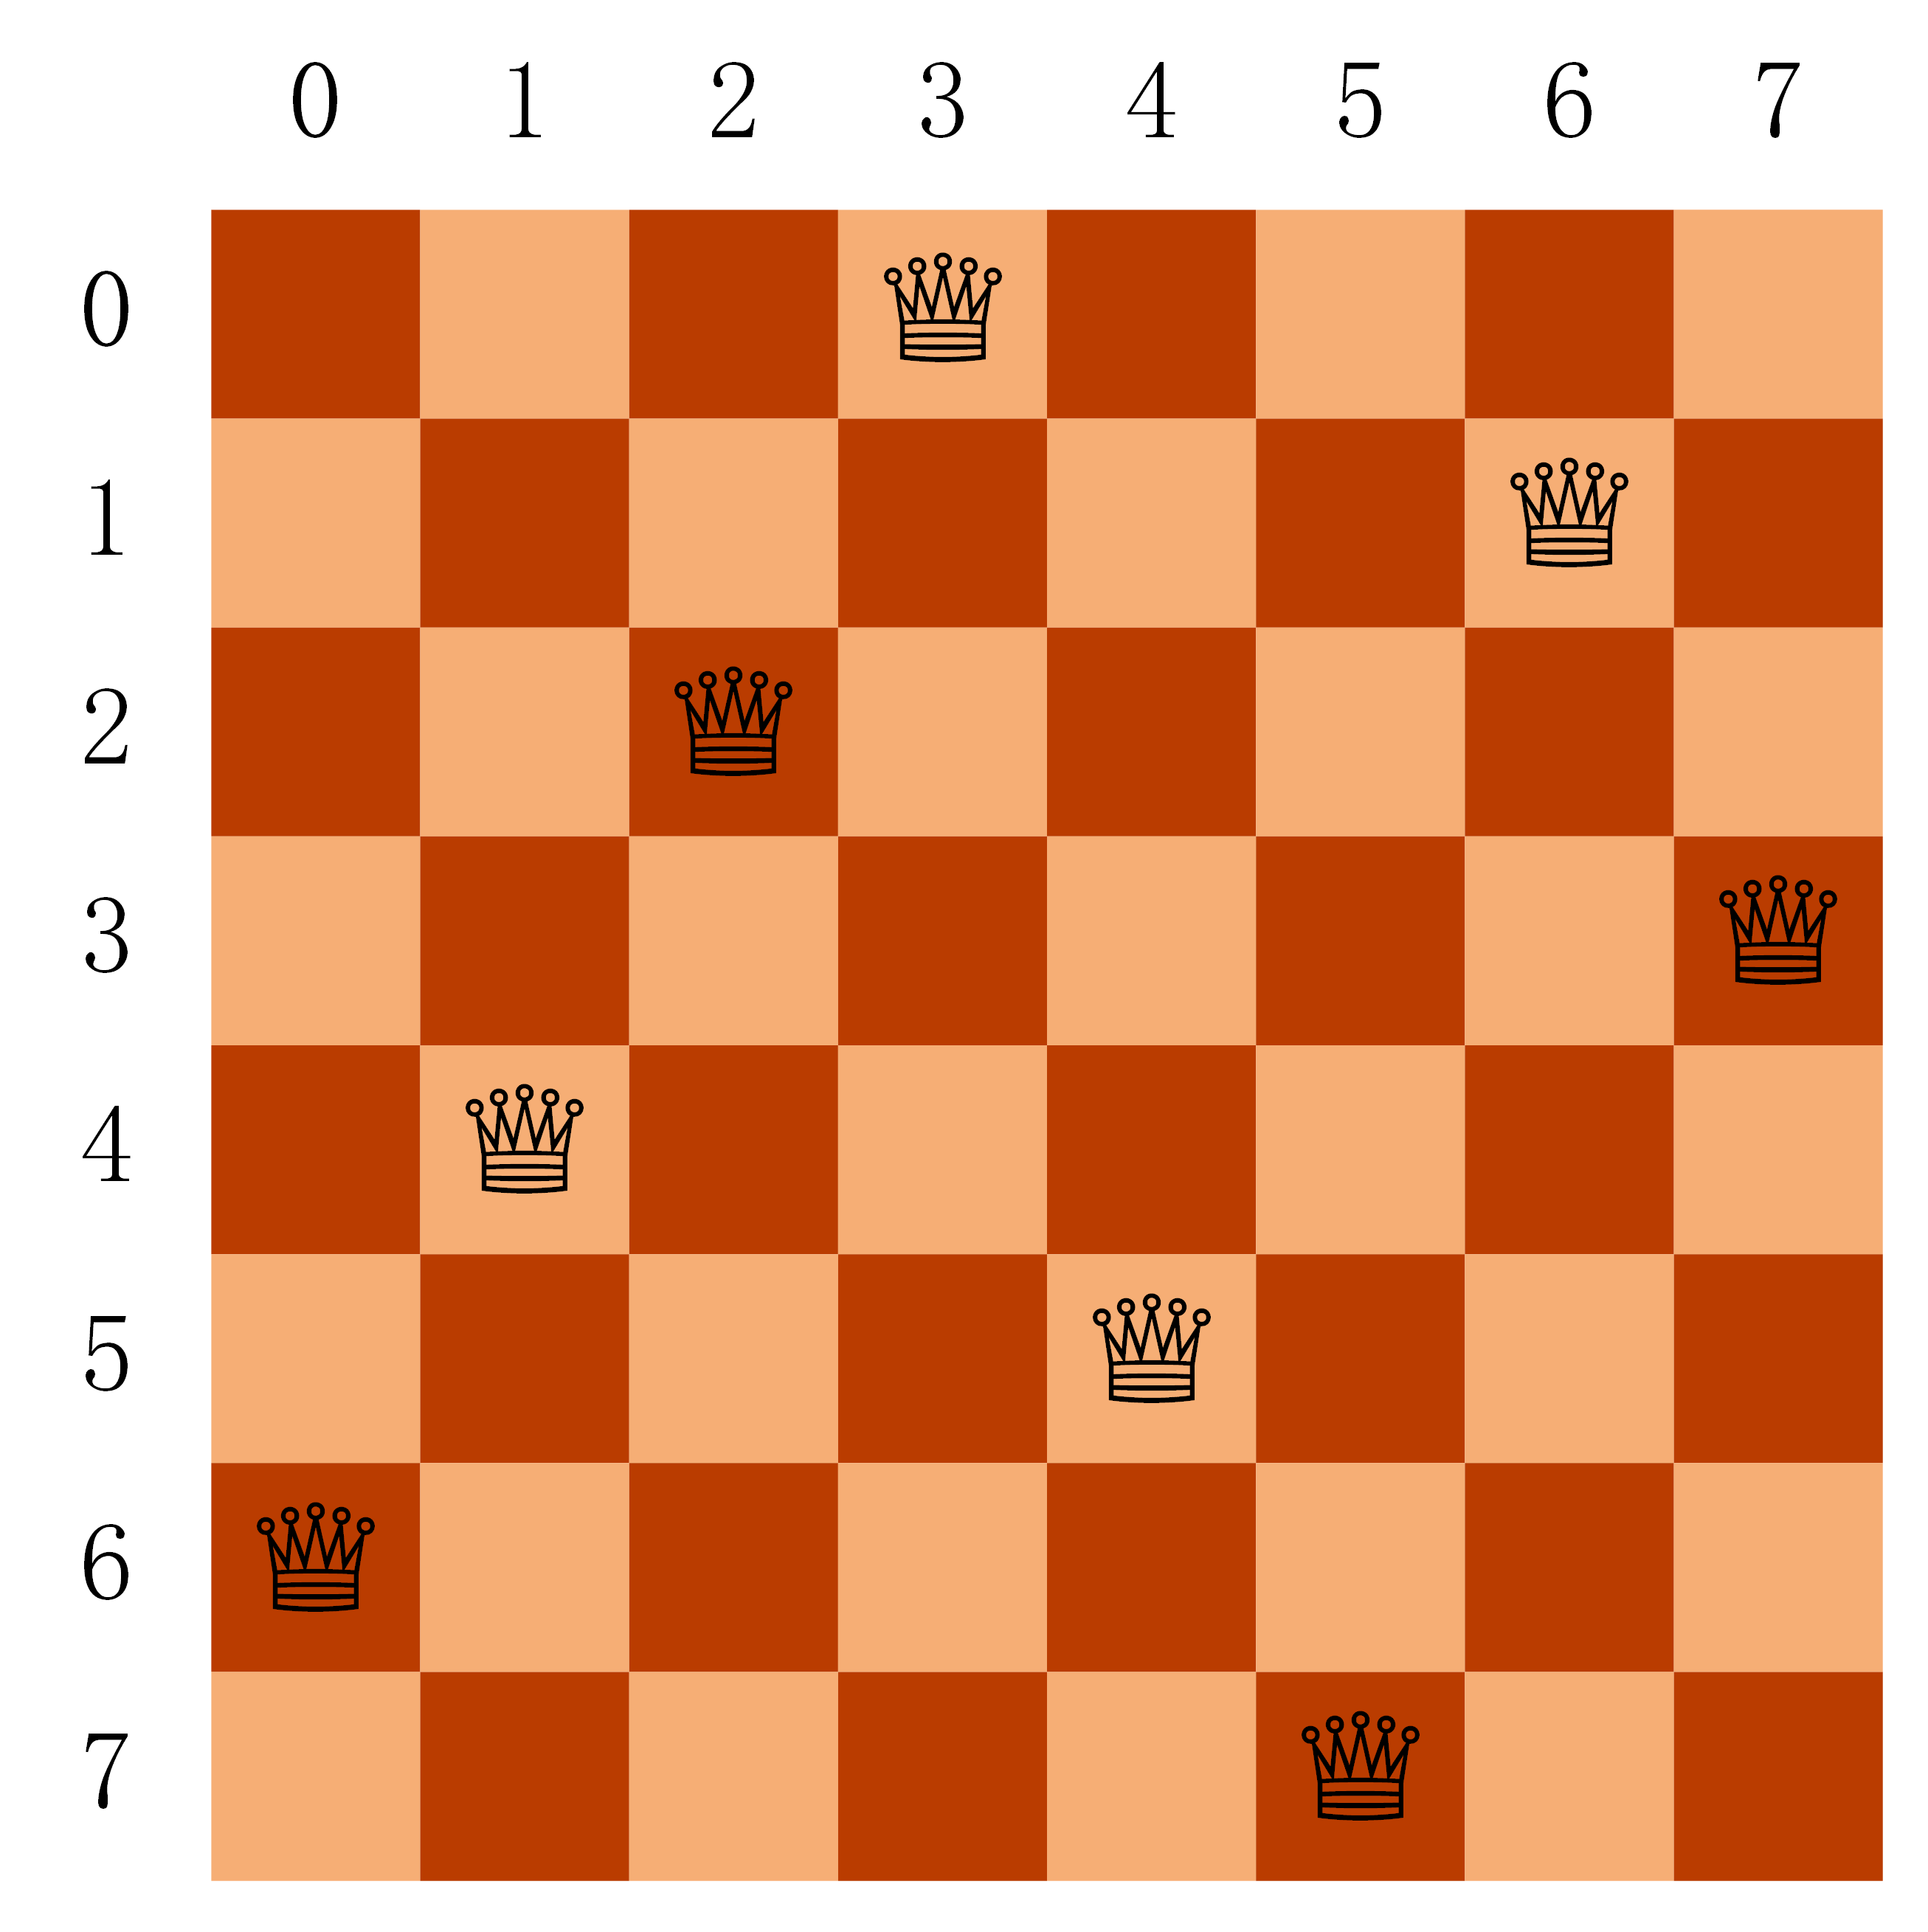
\includegraphics[scale=0.4]{Fig4-3.png}
        \end{figure}
    \end{column}
\end{columns}

\end{frame}



\begin{frame}[fragile]
	%\frametitle{4.3 数组\small{—访问数组元素}}
	% \framesubtitle{——访问数组元素}
\vspace{-5mm}
	\begin{exampleblock}{}%代码清单4.2,例4.2:
		% \begin{minipage}[t]{0.4\linewidth}
		\begin{lstlisting}[numbers=left,numberstyle=\small,numbers=left,xleftmargin=2em,framexleftmargin=2em,basicstyle=\footnotesize\ttfamily]
int main() {
    constexpr int sz = 8;
    int que[sz] = { 0 };//每一行皇后都从第0列开始摆放
    int i = 0;//从第0行开始摆放
    while (i >= 0){
        int k = 0;
        while (k<i){ //检查前面所有皇后是否和第i行皇后冲突
            if(que[k]!=que[i]&&(abs(que[i]-que[k])!=abs(i-k))) ++k;
            else   break;//第k行和第i行皇后产生冲突,退出,转到第11行
        }
        if (k < i) {//检测到冲突
            ++que[i];//处理冲突:移动第i行皇后到当前位置的下一列
            while (que[i] == sz){ //当前行所有尝试都失败,需要回溯
                que[i] = 0; //重置当前行皇后位置
                --i;//回溯到上一行
                if (i < 0) break; //如果回溯到第0行之前,结束运行,转到第19行
                ++que[i];//前一行皇后后移一列
            }
            continue; //重新检测是否与前面已安排皇后冲突,转到第5行
        }else { //没有检测到冲突,安排下一行皇后
            ++i;//移动到下一行
            if (i < sz)  continue; //安排下一行皇后,已安排在第0列,转到第5行
            for (k = 0; k<sz; ++k)   cout << que[k]; //找到一个方案并输出
            break; //结束运行
        }
    }
    return 0;
}
        \end{lstlisting}\ttfamily
	\end{exampleblock}
\end{frame}

\subsection{多维数组}
\begin{frame}[fragile]
	\frametitle{4.3 数组\small{—多维数组}}
	% \framesubtitle{——多维数组}
	\begin{block}{多维数组}
		多维数组指的是数组中的元素类型为数组类型。
		\begin{itemize}
			\item 二维数组
			      \begin{lstlisting}[basicstyle=\small\ttfamily]
int a2d[3][5];
            \end{lstlisting}
			\item 三维数组
			      \begin{lstlisting}[basicstyle=\small\ttfamily]
int a3d[2][3][5];
            \end{lstlisting}
		\end{itemize}
		无论有多少维数,数组元素都存放在一段连续的内存空间。一维数组可以对应数学中的向量,二维数组可对应矩阵。
	\end{block}
\end{frame}

\begin{frame}[fragile]
	\frametitle{4.3 数组\small{—多维数组}}
	% \framesubtitle{——多维数组}
	\begin{block}{多维数组初始化}
		\small{
			\begin{itemize}
				\item 用\alert{列表方式初始化}多维数组\\
				      \texttt{如}:
				      \begin{lstlisting}[basicstyle=\small\ttfamily]
int a2d[3][5] = {
    {0, 1, 2, 1, 4},
    {7, 5, 4, 5, 7},
    {0, 8, 5, 2, 9}};
                      \end{lstlisting}
				\item 内嵌的花括号可以省略:
				      \begin{lstlisting}[basicstyle=\small\ttfamily]
int a2d[3][5] = {0, 1, 2, 1, 4, 7, 5, 4, 5, 7, 0, 8, 5, 2, 9};
                \end{lstlisting}
			\end{itemize}}
	\end{block}
\end{frame}

\begin{frame}[fragile]
	\frametitle{4.3 数组\small{—多维数组}}
	% \framesubtitle{——多维数组}
	\begin{block}{多维数组初始化}
		\small{
			\begin{itemize}
				\item 显式初始化部分数组元素:
				      \begin{lstlisting}[basicstyle=\small\ttfamily]
int a2d[3][5] = {0, 1, 2};
                \end{lstlisting}
				\item 显式初始化每个一维数组中的第一个元素:
				      \begin{lstlisting}[basicstyle=\small\ttfamily]
int a2d[3][5] = {{0}, {1}, {2}};
                \end{lstlisting}
				\item 通过列表元素让编译器自动推断第一维长度:
				      \begin{lstlisting}[basicstyle=\small\ttfamily]
int a2d[][5] = {0, 1, 2, 1, 4, 7, 5, 4, 5, 7, 0, 8};
                \end{lstlisting}
				      或者:\\
				      \begin{lstlisting}[basicstyle=\small\ttfamily]
int a2d[][5] = {{0}, {1}, {2}};
                \end{lstlisting}
			\end{itemize}}
	\end{block}
\end{frame}

\begin{frame}[fragile]
	\frametitle{4.3 数组\small{—多维数组}}
	% \framesubtitle{——多维数组}
	\begin{exampleblock}{练习:}
		\ttfamily 以下不能对二维数组a进行正确初始化的是?\\
		A. int a[2][3] = \{ 0 \};\\
B. int a[][3] = \{ \{ 1,2 \},\{ 0 \} \};\\
		C. int a[2][3] = \{ \{ 1,2 \},\{ 3,4 \},\{ 5,6 \} \};\\
		D. int a[][3] = \{ 1,2,3,4,5,6 \};\\
		\onslide<2->{答案:C}
	\end{exampleblock}
\end{frame}


\begin{frame}[fragile]
	\frametitle{4.3 数组\small{—多维数组}}
	% \framesubtitle{——多维数组}
	\begin{block}{访问多维数组元素}
		\begin{itemize}
			\item 利用下标运算符访问:
			      \begin{lstlisting}[basicstyle=\small\ttfamily]
int a2d[2][2] = {
    {1,2},
    {3,4}};
int val = a2d[1][1];
cout << "val=" << val << endl;//输出val= 4
            \end{lstlisting}
			\item 用嵌套的\texttt{for}语句访问:
			      \begin{lstlisting}[basicstyle=\small\ttfamily]
int a2d[2][2] = {{1,2},{3,4}};
for (int i = 0; i < 2; i++) {
    for (int j = 0; j < 2; j++) {
        cout << "a2d[" << i << "][" << j << "]: ";
        cout << a2d[i][j] << endl;
    }
}
            \end{lstlisting}
		\end{itemize}
	\end{block}
\end{frame}

\begin{frame}[fragile]
	\frametitle{4.3 数组\small{—多维数组}}
	% \framesubtitle{——多维数组}
	\begin{block}{访问多维数组元素}
		\begin{itemize}
			\item 用范围\texttt{~for~}语句访问:
			      \begin{lstlisting}[basicstyle=\small\ttfamily]
int a2d[2][2] = { { 1,2 },{ 3,4 } };
for (auto &row : a2d) {
    for (auto &col : row)
        cout << col << " ";
    cout << endl;
}
            \end{lstlisting}
		\end{itemize}
	\end{block}
\end{frame}

\begin{frame}[fragile]
	\frametitle{4.3 数组\small{—多维数组}}
	% \framesubtitle{——多维数组}
	\ttfamily
	\begin{exampleblock}{练习:}
		1.以下程序的输出结果是?
		\begin{lstlisting}[basicstyle=\small\ttfamily]
int a[][3] = { { 1,2 },{ 0 } };
for (auto &row : a) {
    for (auto &col : row)
        cout << col << " ";
    cout << endl;
}
        \end{lstlisting}
		\onslide<2->{答案:\\1~2~0\\0~0~0}
	\end{exampleblock}
\end{frame}

\begin{frame}[fragile]
	\frametitle{4.3 数组\small{—多维数组}}
	% \framesubtitle{——多维数组}
	\begin{alertblock}{注意}
		\begin{itemize}
			\item 除了最内层的循环外,其它各层循环中必须使用引用,例如:
			      \begin{lstlisting}[basicstyle=\small\ttfamily]
int a2d[2][2] = { { 1,2 },{ 3,4 } };
for (auto &row : a2d) {//row被推导为int(&)[5] 类型
    for (auto col : row) //正确,row为一维数组的引用
        cout << col << " ";
    cout << endl;
}
        \end{lstlisting}
			\item 省去\texttt{row}前面的\texttt{\&},无法通过编译:
			      \begin{lstlisting}[basicstyle=\small\ttfamily]
int a2d[2][2] = { { 1,2 },{ 3,4 } };
for (auto row : a2d) { //row 被推导为int *类型
    for (auto col : row) //错误:row不是列表类型,不能使用范围 for
        cout << col << " ";
    cout << endl;
}
        \end{lstlisting}
		\end{itemize}
	\end{alertblock}
\end{frame}

\begin{frame}[fragile]
	\frametitle{4.3 数组\small{—多维数组}}
	% \framesubtitle{——多维数组}
	\begin{exampleblock}{例4.3:}
		\ttfamily
		打印扫雷游戏的地图。在一个~$n\times n$~网格化的地图上,随机分布一些地雷,要求在每个没有设置地雷的网格内标记出其相邻区域内地雷的数目,每个网格相邻区域只包括同一行和同一列紧邻的4个网格。\\
	\end{exampleblock}
	\begin{center}
		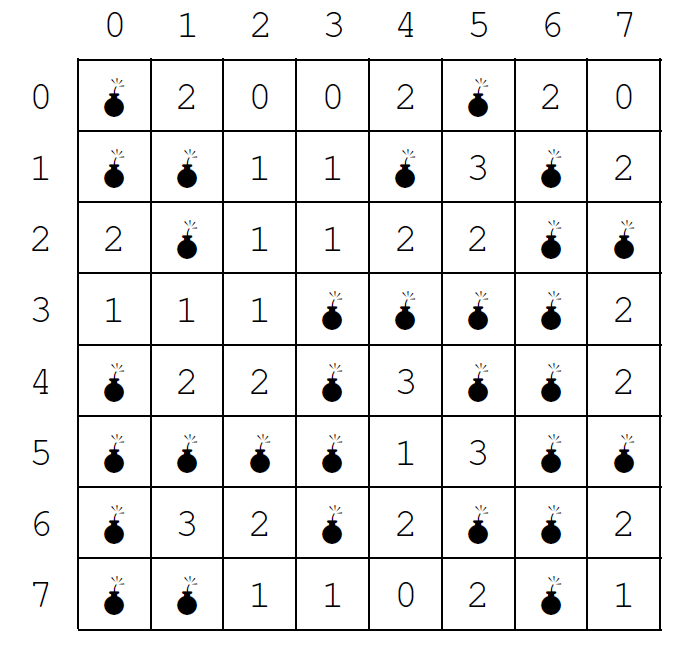
\includegraphics[width=0.4\textwidth]{Fig4-4.png}
	\end{center}
\end{frame}

\begin{frame}[fragile]
	\frametitle{4.3 数组\small{—多维数组}}
	% \framesubtitle{——访问数组元素}
	\begin{exampleblock}{代码清单4.3,例4.3:}
		% \begin{minipage}[t]{0.4\linewidth}
		\begin{lstlisting}[numbers=left,numberstyle=\small,numbers=left,xleftmargin=2em,framexleftmargin=2em,basicstyle=\small\ttfamily]
using namespace std;
int main() {
    srand(time(0));
    constexpr int sz = 8;
    char map[sz][sz];
    for (auto &row : map)     //每个元素的引用
        for (auto &col : row) //内嵌数组中每个元素的引用
            int num = rand() % 100;
            if (num <= 40)    //以0.4的概率设置每个方格的地雷
                col = '*';
            else
                col = '0';    //没有地雷的方格初始化为字符0
        }
    }
        \end{lstlisting}\ttfamily
	\end{exampleblock}
\end{frame}

\begin{frame}[fragile]
	\frametitle{4.3 数组\small{—多维数组}}
	% \framesubtitle{——访问数组元素}
	\begin{exampleblock}{代码清单4.3,例4.3:}
		% \begin{minipage}[t]{0.4\linewidth}
		\begin{columns}
			\begin{column}{0.04\linewidth}
			\end{column}
			\begin{column}{0.96\textwidth}
				\begin{lstlisting}[numbers=left,numberstyle=\small,numbers=left,firstnumber=15,basicstyle=\small\ttfamily]
for (int i = 0; i < sz; ++i) {
    for (int j = 0; j < sz; ++j) {
        if (map[i][j] != '*')
            continue;          //跳过地雷的方格
        if (i + 1 < sz && map[i + 1][j] != '*') map[i + 1][j] += 1;
        if (i - 1 >= 0 && map[i - 1][j] != '*') map[i - 1][j] += 1;
        if (j + 1 < sz && map[i][j + 1] != '*') map[i][j + 1] += 1;
        if (j - 1 >= 0 && map[i][j - 1] != '*') map[i][j - 1] += 1;
    }
}
for (int i = 0; i < sz; ++i) {
    for (int j = 0; j < sz; ++j) {
        cout << map[i][j]<<" ";
    }
    cout << endl;
}
return 0;}
        \end{lstlisting}\ttfamily
			\end{column}
		\end{columns}
	\end{exampleblock}
\end{frame}

\section{指针和数组}
\subsection{指针指向数组}
\begin{frame}[fragile]
	\frametitle{4.4 指针和数组\small{—指针指向数组}}
	% \framesubtitle{——指针指向数组}
	\begin{block}{指针和数组的关系}
		\begin{itemize}
			\item 数组名被转换成数组第一个元素的地址
			      \begin{lstlisting}[basicstyle=\small\ttfamily]
int arr[] = {1, 2, 3, 4, 5};
int *p = arr; //arr被转换成arr[0]的地址
            \end{lstlisting}
			      第二句等价于:
			      \begin{lstlisting}[basicstyle=\small\ttfamily]
int *p = &arr[0];
                \end{lstlisting}
		\end{itemize}
	\end{block}
	\begin{exampleblock}{练习:}
		\ttfamily 对于以下程序段:
		\begin{lstlisting}[basicstyle=\small\ttfamily]
int a[3] = { 5,7,3 };
cout << &a[0] << endl;
        \end{lstlisting}
		若数组a的第二个元素的地址为02F602FFA8C,则该程序的输出为?\\
		\onslide<2->{答案:02F602FFA88}
	\end{exampleblock}
\end{frame}

\begin{frame}[fragile]
	\frametitle{4.4 指针和数组\small{—指针指向数组}}
	% \framesubtitle{——指针指向数组}
	\begin{block}{指针和数组的关系}
		\begin{itemize}
			\item 利用\textcolor[rgb]{0,0,1}{\texttt{auto}}进行类型推导,得到的是一个指针
			      \begin{lstlisting}[basicstyle=\small\ttfamily]
int arr[] = {1, 2, 3, 4, 5};
auto pa = arr; //pa 为int * 类型,显然是一个指针
cout << *pa;     //输出arr[0] 的值1
                \end{lstlisting}
			\item 利用\textcolor[rgb]{0,0,1}{\texttt{decltype}}定义新数组时,数组名\texttt{arr}不会转换为指针
			      \begin{lstlisting}[basicstyle=\small\ttfamily]
decltype (arr) ar2; //ar2 为存放5 个整型数的一维数组
            \end{lstlisting}
		\end{itemize}
	\end{block}
\end{frame}


\begin{frame}[fragile]
	\frametitle{4.4 指针和数组\small{—指针指向数组}}
	% \framesubtitle{——指针指向数组}
	\begin{block}{指针和数组的关系}
		\begin{itemize}
			\item 可用指针指向多维数组\\
			      \begin{lstlisting}[basicstyle=\small\ttfamily]
int a2d[3][5];
int (*p2d)[5] = a2d; //指向a2d 的第一个元素
            \end{lstlisting}
			      \textcolor[rgb]{1,0,0}{提示}:上面的指针定义中,圆括号不能省略,如:
			      \begin{lstlisting}[basicstyle=\small\ttfamily]
int *p2d[5];//p2d是一个含有5个指向整型对象的指针数组
            \end{lstlisting}
		\end{itemize}
	\end{block}
\end{frame}

\begin{frame}[fragile]
	\frametitle{4.4 指针和数组\small{—指针指向数组}}
	% \framesubtitle{——指针指向数组}
	\begin{block}{数组名和指针对象的关系}
		一个数组名可理解为一个\texttt{const}指针,但两者并不完全等价\\
		\texttt{如:}\\
		\begin{lstlisting}[basicstyle=\small\ttfamily]
int * const p = &arr[0]; //arr 可以理解为const 指针p
cout << sizeof(arr) << " " << sizeof(p);
        \end{lstlisting}
		使用运算符\texttt{~sizeof}测试的输出结果为:20 4,分别为一个含有5个整型元素的数组和一个指向整型类型的指针对象的大小
	\end{block}
\end{frame}

\subsection{通过指针访问数组}
\begin{frame}[fragile]
	\frametitle{4.4 指针和数组\small{—利用指针访问数组}}
	% \framesubtitle{——利用指针访问数组}
	\begin{block}{利用指针访问数组}
		对于如下数组和指针:
		\begin{lstlisting}[basicstyle=\small\ttfamily]
int arr[] = {1, 2, 3, 4, 5};
int *p = arr; //p 指向数组arr
        \end{lstlisting}
		示意图如下图所示:
	\end{block}
	\begin{center}
		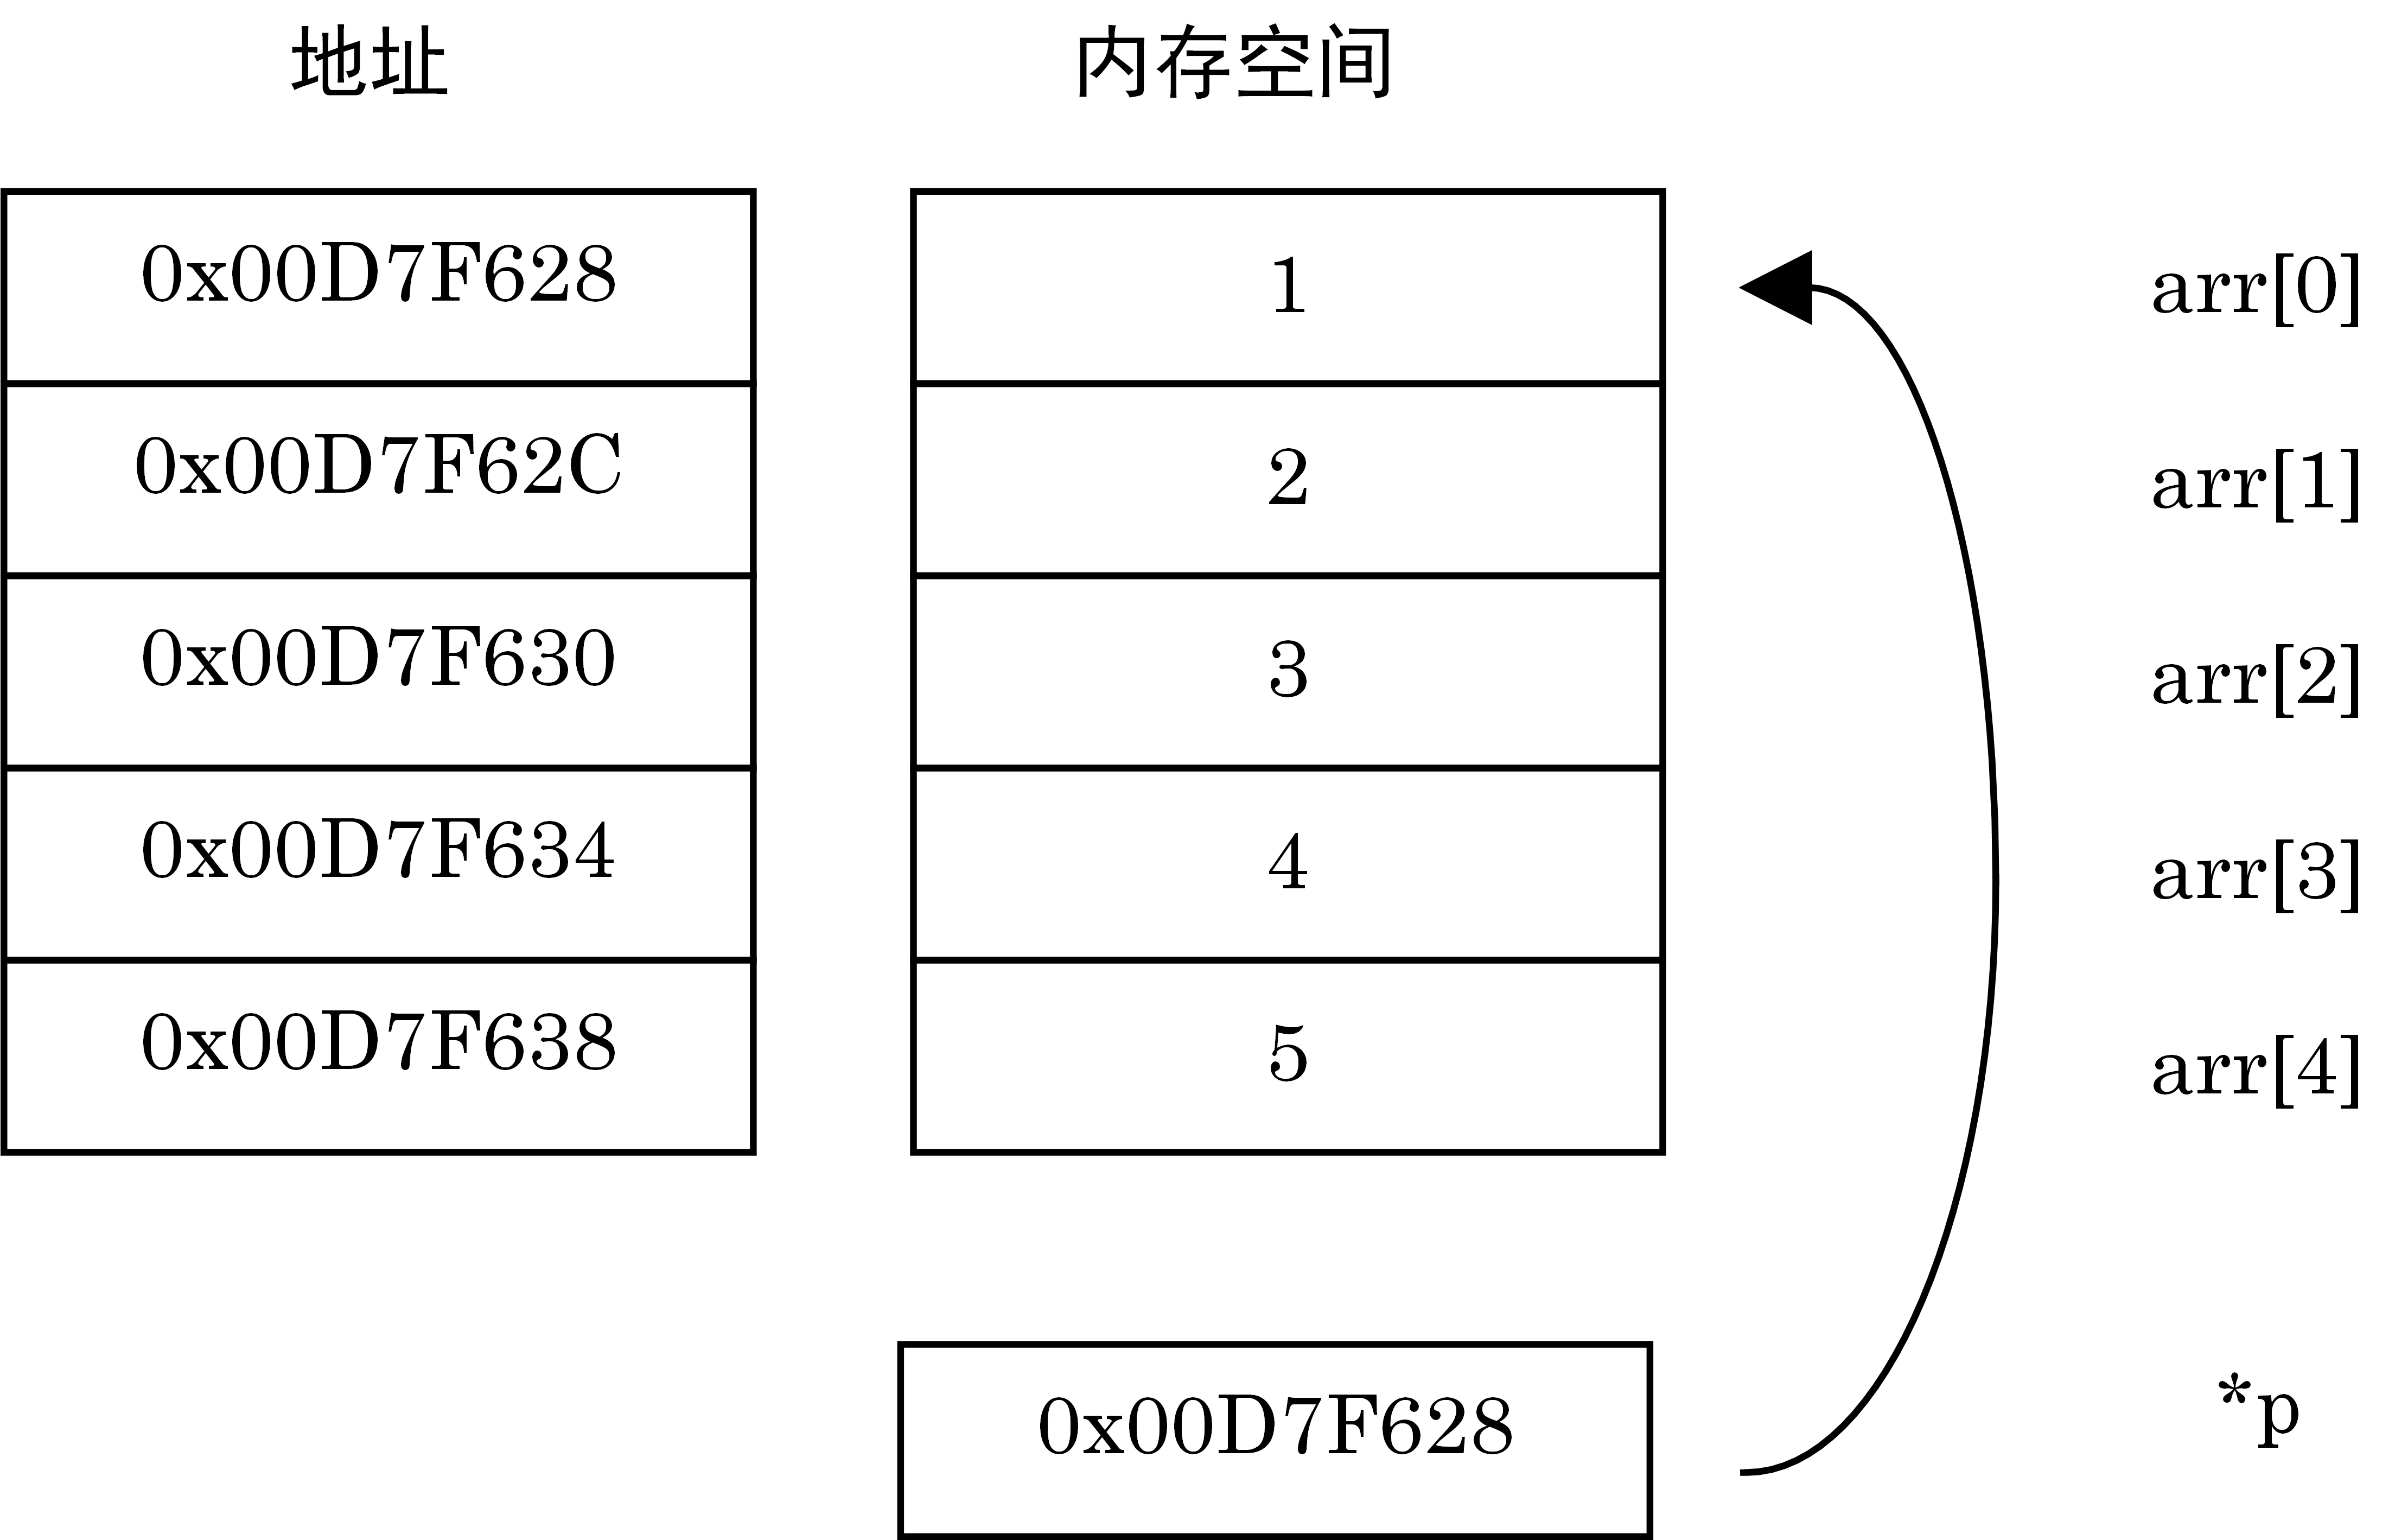
\includegraphics[scale=0.3]{pointer_array.png}
	\end{center}
\end{frame}

\begin{frame}[fragile]
	\frametitle{4.4 指针和数组\small{—利用指针访问数组}}
	% \framesubtitle{——利用指针访问数组}
	\begin{block}{利用指针访问数组}
		当指针和数组数组关联时,\texttt{C++}支持如下指针运算:
		\begin{itemize}
			\item 指针的移动
			      \begin{lstlisting}[basicstyle=\small\ttfamily]
int arr[] = {1, 2, 3, 4, 5};
int *p = arr;       //p指向数组arr
int *p2 = p + 3; //返回p后面第3 个元素的地址,即&arr[3]
int *p3 = p++;      //p后移一个位置,p3指向p原来的位置&arr[0]
int *p4 = ++p;      //p继续后移一个位置,p4和p指向同一个位置&arr[2]
            \end{lstlisting}
			\item 关系运算\\
			      \texttt{p == p4, p4 > p3, p3 <= p2}等都为真。
			\item 指针相减\\
			      两个指针相减的结果为所指向数组元素的位置距离,比如表达式\alert{\texttt{p4-p3}}的结果为2。
		\end{itemize}
	\end{block}
\end{frame}

\begin{frame}[fragile]
	\frametitle{4.4 指针和数组\small{—利用指针访问数组}}
	% \framesubtitle{——利用指针访问数组}
	\begin{block}{关于指针运算需注意:}
		\begin{itemize}
			\item \textcolor[rgb]{1,0,0}{指针}在运算的过程中\textcolor[rgb]{1,0,0}{不能越界}。第一个元素到最后一个元素的下一个位置为有效位置,比如:
			      \begin{lstlisting}[basicstyle=\small\ttfamily]
p2 = &arr[0]; //正确:指向第一个元素,等价于p2 = arr;
p2 = &arr[5]; //正确:指向尾元素后面的一个位置,等价于p2=arr + 5;
            \end{lstlisting}
			      虽然不存在元素\texttt{arr[5]},但可以计算该位置的地址。
			\item 仅当两个指针指向同一个数组时,它们之间的运算才有意义。
		\end{itemize}
	\end{block}
\end{frame}

\begin{frame}[fragile]
	\frametitle{4.4 指针和数组\small{—利用指针访问数组}}
	% \framesubtitle{——利用指针访问数组}
	\begin{block}{利用指针访问数组:}
		\begin{lstlisting}[basicstyle=\small\ttfamily]
int arr[] = {1, 2, 3, 4, 5};
int *p = arr;               //p 指向数组 arr
int val = *(p + 2) + 1; //等价于 int val = arr[2] + 1;
int val2 = p[2];            //等价于 int val2 = arr[2];
            \end{lstlisting}
	\end{block}
\end{frame}

\begin{frame}[fragile]
	\frametitle{4.4 指针和数组\small{—利用指针访问数组}}
	% \framesubtitle{——利用指针访问数组}
	\begin{block}{利用指针访问二维数组}
		\begin{lstlisting}[basicstyle=\small\ttfamily]
int a2d[3][5] = { { 0 },{ 0 },{ 0 } };
int(*p2d)[5] = a2d;
cout << a2d[1][1] << endl;//输出为0
p2d[1][1] = 1;
cout << a2d[1][1] << endl;//输出为1
        \end{lstlisting}
		\texttt{p2d[1][1]}与下面代码等价:\\
		\texttt{*(*(p2d + 1) + 1) = 1;~~~~~~*(*(a2d + 1) + 1) = 1;\\
			*(p2d[1] + 1) = 1; ~~~~~~~~~*(a2d[1] + 1) = 1;}
	\end{block}
\end{frame}

\begin{frame}[fragile]
	\frametitle{4.4 指针和数组\small{—利用指针访问数组}}
	% \framesubtitle{——利用指针访问数组}
	\begin{block}{利用\texttt{auto}简化代码}
		\begin{lstlisting}[basicstyle=\small\ttfamily]
int a2d[3][5] = { { 1 },{ 1 },{ 1 } };
for (auto p = a2d; p < a2d + 3; ++p) {//p的类型为int (*)[5]
    for (auto q = *p; q < *p + 5; ++q) {//q的类型为int *
        cout << *q << " ";
    }
    cout << endl;
}
        \end{lstlisting}
		\ttfamily 输出为:\\
		1~0~0~0~0\\
		1~0~0~0~0\\
		1~0~0~0~0\\
	\end{block}
\end{frame}


\begin{frame}[fragile]
	\frametitle{4.4 指针和数组\small{—利用指针访问数组}}
	% \framesubtitle{——利用指针访问数组}
	\begin{block}{利用数组元素连续的特性遍历数组:}
		\begin{lstlisting}[basicstyle=\small\ttfamily]
int a2d[3][5] = { { 1 },{ 1 },{ 1 } };
for (auto p = &a2d[0][0]; p < a2d[0] + 15; ++p) {
    if ((p - a2d[0]) % 5 == 0) //a2d[0] 等价于 &a2d[0][0]
        cout << endl; //每打印5个元素后换行
    cout << *p << " ";
}
        \end{lstlisting}
		\ttfamily 输出为:\\
		1~0~0~0~0\\
		1~0~0~0~0\\
		1~0~0~0~0\\
	\end{block}
\end{frame}

\section{string 类型}


\begin{frame}[fragile]
	\frametitle{4.5 \texttt{string}类型}
	% \framesubtitle{——if 语句}
	\begin{abstractblock}{\texttt{string}类型是\texttt{C++}标准库类型}
		支持变长的字符串和常用的字符串操作。
	\end{abstractblock}
	\begin{abstractblock}{\texttt{using}声明}
		如下声明来引入单个名字:
		\begin{lstlisting}[basicstyle=\small\ttfamily]
using std::cin;
                \end{lstlisting}
		一劳永逸地引入\texttt{std}命名空间内所有的名字:
		\begin{lstlisting}[basicstyle=\small\ttfamily]
using namespace::std;
                \end{lstlisting}
	\end{abstractblock}
\end{frame}
\subsection{string类型定义和常用操作}
\begin{frame}[fragile]
	\frametitle{\texttt{string}类型\small{—定义和初始化\texttt{string}对象}}
	% \framesubtitle{——定义和初始化\texttt{string}对象}
	\begin{block}{定义\texttt{string}类型}
		\begin{lstlisting}[basicstyle=\small\ttfamily]
string str1;                //默认初始化,定义一个空字符串
string str2(str1);          //等价于string str2 = str1; str2是str1的一个拷贝
string str3 = "Rosita"; //复制初始化
string str4("Rosita");      //直接初始化
string str5(5, ’R’);      //直接初始化,str5 的内容为 RRRRR
        \end{lstlisting}
	\end{block}
\end{frame}

\begin{frame}[fragile]
	\frametitle{4.5 \texttt{string}类型\small{—\texttt{string}类型常用操作}}
	% \framesubtitle{——\texttt{string}类型常用操作}
	\begin{block}{\texttt{string}对象的输入和输出}
		\begin{lstlisting}[basicstyle=\small\ttfamily]
string s;
cin >> s;    //遇到空白字符停止
cout << s; //输出s的内容
                \end{lstlisting}
		利用\texttt{getline}函数读取空白字符:
		\begin{lstlisting}[basicstyle=\small\ttfamily]
getline(cin, s);
                    \end{lstlisting}
		\texttt{当输入"hello C++ "时(注意里面的空格),s~的内容为"hello C++ }"。
	\end{block}
\end{frame}

\begin{frame}[fragile]
	\frametitle{4.5 \texttt{string}类型\small{—\texttt{string}类型常用操作}}
	% \framesubtitle{——\texttt{string}类型常用操作}
	\begin{block}{\texttt{string}对象的大小}
		\begin{lstlisting}[basicstyle=\small\ttfamily]
string s;
cin >> s;
cout << s.size() << endl;//输出 s 里面字符的个数,与 s.length() 等价
if(!s.empty())               //如果 s 非空,则输出其内容
    cout << s;
                \end{lstlisting}
		调用类的成员函数需在对象名后加\alert{\texttt{.}}操作符。指针对象需用\alert{\texttt{->}}操作符:
		\begin{lstlisting}[basicstyle=\small\ttfamily]
string *ps = &s;                 //定义一个指针对象指向 string 对象 s
cout << ps->size() << endl; //通过指针调用 size 成员函数
                \end{lstlisting}
	\end{block}
\end{frame}


\begin{frame}[fragile]
	\frametitle{4.5 \texttt{string}类型\small{—\texttt{string}类型常用操作}}
	% \framesubtitle{——\texttt{string}类型常用操作}
	\begin{block}{\texttt{string}对象的关系运算}
		\alert{比较规则}:如果两个\texttt{string}对象长度不一样,且较短的\texttt{string}对象和较长的对象前面的每个字符都一样,则较短的\texttt{string}对象小于较长的\texttt{string}对象;否则返回相同位置上第一对不同字符的比较结果(\alert{字典排序靠前的字符小}),例如:\\
		\begin{lstlisting}[basicstyle=\small\ttfamily]
string s1 = "Hello C++";
string s2 = "Hello";
string s3 = "Hi";
                    \end{lstlisting}
		依据上述规则,\texttt{s1}大于\texttt{s2},\texttt{s2}小于\texttt{s3}。
	\end{block}
	\begin{block}{\texttt{string}对象的加法运算}
		\begin{lstlisting}[basicstyle=\small\ttfamily]
string s1 = "Hello ", s2 = "C++";
string s3 = s1 + s2;
s1 += s2;                      //s3和s1的内容都是"Hello C++"
string s4 = "Hello " + s2;//string对象可与字面值常量相加
                \end{lstlisting}
	\end{block}
\end{frame}

\begin{frame}[fragile]
	\frametitle{4.5 \texttt{string}类型\small{—\texttt{string}类型常用操作}}
	% \framesubtitle{——\texttt{string}类型常用操作}
	\begin{block}{访问单个字符}
		\begin{itemize}
			\item 利用下标运算和\alert{\texttt{at}函数}访问单个字符
			      \begin{lstlisting}[basicstyle=\small\ttfamily]
string s = "hello";
s[1] = 'H'; //对第二个元素进行写操作
cout << s.at(1) << endl;
        \end{lstlisting}
			      下标运算和 \texttt{at} 函数都要求一个有效的位置值,最小值为0,最大值为对象的长度-1。利用\alert{\texttt{at}}成员函数访问是安全的,它会自动\alert{检查}位置的\alert{合法性}\\
			\item 利用\alert{\texttt{front}}和\alert{\texttt{back}}操作访问第一个和最后一个字符:
			      \begin{lstlisting}[basicstyle=\small\ttfamily]
cout << s.front() << " " << s.back() << endl; //打印输出h o
        \end{lstlisting}
		\end{itemize}
	\end{block}
\end{frame}

\begin{frame}[fragile]
	\frametitle{4.5 \texttt{string}类型\small{—\texttt{string}类型常用操作}}
	% \framesubtitle{——\texttt{string}类型常用操作}
	\begin{exampleblock}{例4.4:}
		\ttfamily
		猜单词游戏,其中一个玩家给定一个单词,让另外一个玩家猜。\alert{规则如下}:每次猜测单词里面可能的一个字母,并给定猜错的最大次数,比如3次。每次猜测要给出相关提示,包括猜测的字母是否正确、字母是否已经猜测过、剩余机会次数以及当前猜测的进度,未猜中的字母用符号*代替。如果在给定的最大猜错次数内正确猜出单词的所有字母,则挑战成功,否则失败。失败时给出单词的全部字母。\label{exam4-4}
	\end{exampleblock}
\end{frame}

\begin{frame}[fragile]
	\frametitle{4.5 \texttt{string}类型\small{—\texttt{string}类型常用操作}}
	% \framesubtitle{——\texttt{string}类型常用操作}
	\begin{exampleblock}{代码清单4.4,例4.4:}
		\begin{lstlisting}[numbers=left,numberstyle=\small,numbers=left,xleftmargin=2em,framexleftmargin=2em,basicstyle=\small\ttfamily]
using namespace std;
int main() {
    string target;
    cout << "请给出一个单词:";
    cin >> target;
    cout << string(100, '\n'); //输出100个换行,用来隐藏输入的单词
    int length = target.length();
    string attempt(length,'*'),badchars;//分别记录当前正确和错误的猜测
    int guesses = 5; //最大尝试次数
    cout<<"单词已准备好,它有"<<length<<"个字母:"<<attempt<<endl;
        \end{lstlisting}
	\end{exampleblock}
\end{frame}

\begin{frame}[fragile]
	\frametitle{4.5 \texttt{string}类型\small{—\texttt{string}类型常用操作}}
	% \framesubtitle{——\texttt{string}类型常用操作}
	\begin{exampleblock}{代码清单4.4,例4.4:}
		\begin{lstlisting}[numbers=left,numberstyle=\small,numbers=left,xleftmargin=2em,framexleftmargin=2em,firstnumber=11,basicstyle=\small\ttfamily]
do{
    char letter;
    cout << "请猜测一个字母: ";
    cin >> letter; //badchars或attempt中已有letters
    if (badchars.find(letter) != string::npos ||
        attempt.find(letter) != string::npos)
        cout << "已经猜过该字母,请重猜" << endl;
        continue; //string::npos匹配失败标志位
    }
    auto loc = target.find(letter); //使用auto自动推导loc类型
    if (loc == string::npos) {
        cout << "没有此字母!" << endl;
        --guesses; //允许错误次数-1
        badchars += letter; //猜错的字母放到badchars里
    }
        \end{lstlisting}
	\end{exampleblock}
\end{frame}

\begin{frame}[fragile]
	\frametitle{4.5 \texttt{string}类型\small{—\texttt{string}类型常用操作}}
	% \framesubtitle{——\texttt{string}类型常用操作}
	\begin{exampleblock}{代码清单4.4,例4.4:}
		% \begin{minipage}[t]{0.4\linewidth}
		\begin{lstlisting}[numbers=left,numberstyle=\small,numbers=left,xleftmargin=2em,framexleftmargin=2em,firstnumber=26,basicstyle=\small\ttfamily]
            else {
                cout << "有这个字母,继续加油!" << endl;
                do {//把attempt里面相应的*用猜对的字母替换
                    attempt[loc]=letter;//如果找到了,则下一次搜索从loc+1开始
                    loc = target.find(letter, loc + 1);
                } while (loc != string::npos);
        }
        cout << "你猜测的单词:" << attempt << endl;
        if (attempt != target)
            cout << "剩余" << guesses << " 次猜错机会" << endl;
    } while (guesses > 0 && attempt != target);
    if (guesses > 0)
        cout << " 成功了,恭喜你!" << endl;
    else
        cout<<"对不起,失败了,下次再挑战吧,单词是"<<target<<endl;
}
        \end{lstlisting}\ttfamily
	\end{exampleblock}
\end{frame}

\subsection{C风格字符串}

\begin{frame}[fragile]
	\frametitle{4.5 \texttt{string}类型\small{—\texttt{C}风格字符串}}
	% \framesubtitle{——\texttt{C}风格字符串}
	\begin{block}{\texttt{C}风格字符串}
		\texttt{C}风格字符串不是一种类型,而是以空字符结尾(\texttt{'\textbackslash 0'})的字符数组,例如:
		\begin{lstlisting}[basicstyle=\small\ttfamily]
char cstr[] = "Hello";
        \end{lstlisting}
	\end{block}
	% \texttt{C}风格字符串处理函数:\\
	\begin{table}[h]
		\begin{center}
			% \caption{常用~C~风格字符串处理函数}\color{black}\label{tab4-1}
			\ttfamily
			\begin{tabularx}{\textwidth}{ |Xp{9cm}| }
				\hline
				strlen(s)     & 返回s的长度,不包含结束符'\textbackslash 0'                                                                            \\
				strcmp(s1,s2) & 字符串比较函数。和~C++ string~类型对象相比较的规则一样:如果~s1==s2,返回0;如果~s1>s2,返回正值;如果~s1<s2,返回负值 \\
				strcpy(s1,s2) & 字符串复制函数。将字符串~s2~复制给~s1,返回~s1                                                                         \\
				strcat(s1,s2) & 字符串链接函数。将字符串~s2~附加到~s1~之后,返回~s1                                                                    \\
				\hline
			\end{tabularx}
		\end{center}
	\end{table}
\end{frame}

\begin{frame}[fragile]
	\frametitle{4.5 \texttt{string}类型\small{—\texttt{C}风格字符串}}
	% \framesubtitle{——\texttt{C}风格字符串}
	\begin{block}{利用指针处理\texttt{C}风格字符串}
		\begin{lstlisting}[basicstyle=\small\ttfamily]
char cstr[] = "Hello";
char *ps = cstr;//指向字符数组cstr
char *ps2 = "C++";
cout << ps << "," << ps2 << endl; //输出Hello,C++
        \end{lstlisting}
	\end{block}
\end{frame}

\begin{frame}[fragile]
	\frametitle{4.5 \texttt{string}类型\small{—\texttt{C}风格字符串}}
	% \framesubtitle{——\texttt{C}风格字符串}
	\begin{alertblock}{使用处理\texttt{C}风格字符串的函数时应注意:}
		\begin{itemize}
			\item 每个操作对象必须以空字符\texttt{'\textbackslash 0'}结尾,否则会产生未定义的行为:
			      \begin{lstlisting}[basicstyle=\small\ttfamily]
char cs[] = {’C’, ’+’, ’+’};
cout << strlen(cs) << endl; //错误:cs没有以空字符结束
            \end{lstlisting}
			\item 如果对操作对象进行修改,必须要有足够大的内存空间:
			      \begin{lstlisting}[basicstyle=\small\ttfamily]
char small[] = "C++", big[] = "Programming";
cout << strcpy(small, big) << endl; //错误:small 内存空间不足
            \end{lstlisting}
		\end{itemize}
	\end{alertblock}
\end{frame}


\begin{frame}[fragile]
	\frametitle{4.5 \texttt{string}类型\small{—\texttt{C}风格字符串}}
	% \framesubtitle{——\texttt{C}风格字符串}
	\begin{block}{\texttt{string} 类对象使用 \texttt{C} 风格字符串处理函数}
		需要通过\texttt{string}类成员函数\alert{\texttt{c\_str}}来获取\texttt{string}对象存储的字符串的\alert{首地址},例如:\\
		\begin{lstlisting}[basicstyle=\small\ttfamily]
string str = "hello";
char carr[10];
strcpy(carr, str.c_str());
        \end{lstlisting}
		\texttt{string}~的成员函数~\texttt{c\_str}~返回~\texttt{const char*}~类型的指针,确保其指向的对象不被修改。
	\end{block}
\end{frame}

\begin{frame}[fragile]
	\frametitle{4.6 \texttt{vector}类型}
	% \framesubtitle{——C风格字符串}
	\begin{abstractblock}{\texttt{vector} 类型}
		\begin{itemize}
			\item \texttt{vector}和数组都是有序元素的集合
			\item \texttt{vector}支持\alert{变长操作},容量大小可根据需要动态调整
			\item \texttt{vector}是一种容器类型,能够存放类型相同的元素
			\item 使用\texttt{vector}需要在程序中包含\texttt{vector}头文件:\\
			      \begin{lstlisting}[basicstyle=\small\ttfamily]
#include <vector>
            \end{lstlisting}
		\end{itemize}
	\end{abstractblock}
\end{frame}

\section{vector 类型}
\subsection{vector 类型定义和常用操作}
\begin{frame}[fragile]
	\frametitle{4.6 \texttt{vector}类型\small{—定义和初始化\texttt{vector}对象}}
	% \framesubtitle{——定义和初始化\texttt{vector}对象}
	\begin{table}[h]
		\centering
		\ttfamily\footnotesize{
			\begin{tabularx}{\textwidth}{|Xp{6.5cm}|}\hline
				vector<T> v1               & 定义一个存放~T~类型元素的空对象~v1              \\
				vector<T> v2(v1)           & 复制~v1~里面所有元素到~v2                       \\
				vector<T> v3(n)            & 指定初始元素为~n~个                             \\
				vector<T> v4(n,value)      & 指定~n~个值为~value~的元素                      \\
				vector<T> v5=\{a,b,c,...\} & 采用列表初始化,v5~的元素个数为列表里面值的个数 \\
				vector<T> v6\{a,b,c,...\}  & 等价于~v5=\{a,b,c,...\}                         \\\hline
			\end{tabularx}}
	\end{table}
	\begin{block}{定义\texttt{vector}对象}
		\begin{lstlisting}[basicstyle=\small\ttfamily]
vector<int> v1; //存放整数的空vector
vector<int> v2 = {0,1,2}; //v2有三个元素,值分别为0、1和2
vector<int> v3(10);         //v3可存放10个整数,值为默认值0
vector<int> v4(10,1);       //v4存放10个整数1
vector<string> v5 = {"Hi","Lisha","Mandy","Rosita"};
vector<vector<int>> v6(10,v2);
        \end{lstlisting}
		与数组类似,\texttt{vector}里面的元素也是顺序存放在连续的内存空间内
	\end{block}
\end{frame}

\begin{frame}[fragile]
	\frametitle{4.6 \texttt{vector}类型\small{—\texttt{vector}类型常用操作}}
	% \framesubtitle{——\texttt{vector} 类型常用操作}
	\begin{block}{添加、删除元素}
		\begin{lstlisting}[basicstyle=\small\ttfamily]
vector<int> vi;
for(int i=0; i < 100; ++i)
    vi.push_back(i);//依次添加100个数:0-99
                \end{lstlisting}
		\texttt{vi.push\_back()}成员函数称为尾插,即从容器尾端添加元素\\
		\texttt{vi.pop\_back()}成员函数可从容器尾端移除一个元素\\
		\texttt{vi.clear()}成员函数可移除容器所有元素\\
	\end{block}
	\begin{block}{访问元素}
		可用\alert{下标}运算符或\alert{\texttt{at}}成员函数访问容器里的元素\
		\begin{lstlisting}[basicstyle=\small\ttfamily]
cout << vi.at(1);//或者cout << vi[1];
                \end{lstlisting}
		\texttt{at}函数会自动检查访问位置的合法性而下标运算符不会
	\end{block}
\end{frame}

\subsection{使用迭代器}
\begin{frame}[fragile]
	\frametitle{4.6 \texttt{vector}类型\small{—使用迭代器}}
	% \framesubtitle{——使用迭代器}
	\begin{block}{借助容器的成员函数获取元素迭代器}
		\begin{lstlisting}[basicstyle=\small\ttfamily]
vector<int> vi = {0,1,2,3};
auto itb = vi.begin();//itb 指向 vi 的第一个元素
auto ite = vi.end();//ite 指向 vi 的尾后元素
                \end{lstlisting}
	\end{block}
	\begin{block}{利用解引用获取迭代器指向对象的内容}
		\begin{lstlisting}[basicstyle=\small\ttfamily]
cout << *itb << endl; //输出第一个元素值0
                \end{lstlisting}
	\end{block}
\end{frame}

\begin{frame}[fragile]
	\frametitle{4.6 \texttt{vector}类型\small{—使用迭代器}}
	% \framesubtitle{——使用迭代器}
	\begin{block}{指向\texttt{vector}类型的迭代器支持指针运算}
		\begin{lstlisting}[basicstyle=\small\ttfamily]
for(auto it = vi.begin(); it != vi.end(); ++it){
    *it *= 2; //每个元素乘 2
    cout << *it <<endl;
}
        \end{lstlisting}
		\alert{建议}:在\texttt{for}循环的结束条件中,为了代码的通用性习惯上为迭代器选择\texttt{!=}运算,而不是\texttt{<}运算
	\end{block}
\end{frame}

\begin{frame}[fragile]
	\frametitle{4.6 \texttt{vector}类型\small{—使用迭代器}}
	% \framesubtitle{——使用迭代器}
	\begin{block}{使用成员选择运算符}
		当迭代器指向的元素类型为类类型时,可以用\alert{\texttt{.}}或\alert{\texttt{->}运算符}进行成员选择,例如:\\
		\begin{lstlisting}[basicstyle=\small\ttfamily]
vector<string> vs = {"Hi","Lisha","Mandy","Rosita"};
for(auto it = vs.begin(); it != vs.end(); ++it ){
    cout << (*it).size() << endl;//选择 string 类成员函数 size
}
        \end{lstlisting}
		\textcolor[rgb]{1,0,0}{注意}:迭代器外面的圆括号不可缺少,否则将表达完全不同的意思:\\
		\begin{lstlisting}[basicstyle=\small\ttfamily]
*it.size();//错误:迭代器 it 没有成员函数 size,相当于 *(it.size());
        \end{lstlisting}
	\end{block}
\end{frame}

\begin{frame}[fragile]
	\frametitle{4.6 \texttt{vector}类型\small{—使用迭代器}}
	% \framesubtitle{——使用迭代器}
	\begin{block}{使用\texttt{->}运算符简化表达}
		\begin{lstlisting}[basicstyle=\small\ttfamily]
for(auto it = vs.begin(); it != vs.end(); ++it ){
    cout << it->size() << endl;
}
        \end{lstlisting}
	\end{block}
\end{frame}

\begin{frame}[fragile]
	\frametitle{4.6 \texttt{vector}类型\small{—使用迭代器}}
	% \framesubtitle{——使用迭代器}
	\begin{exampleblock}{例4.5}
		\ttfamily 为例4.3中的扫雷游戏地图中的每个方格编号,编号从0开始,按照从上到下、从左到右的顺序依次编号。例如,第0行第0列编号为0,第0行第1列编号为1,依次类推。\\
		\alert{要求}:若玩家点击的方格无地雷,则找出所有与该方格连通的非雷区。如点击编号为49的方格,则下图中编号下划线的方格都是与之相邻的非雷区\\
		\alert{提示}:采用宽度优先搜索(breadth-first search)策略来求解。
	\end{exampleblock}
	\begin{columns}
		\begin{column}{0.4\linewidth}
			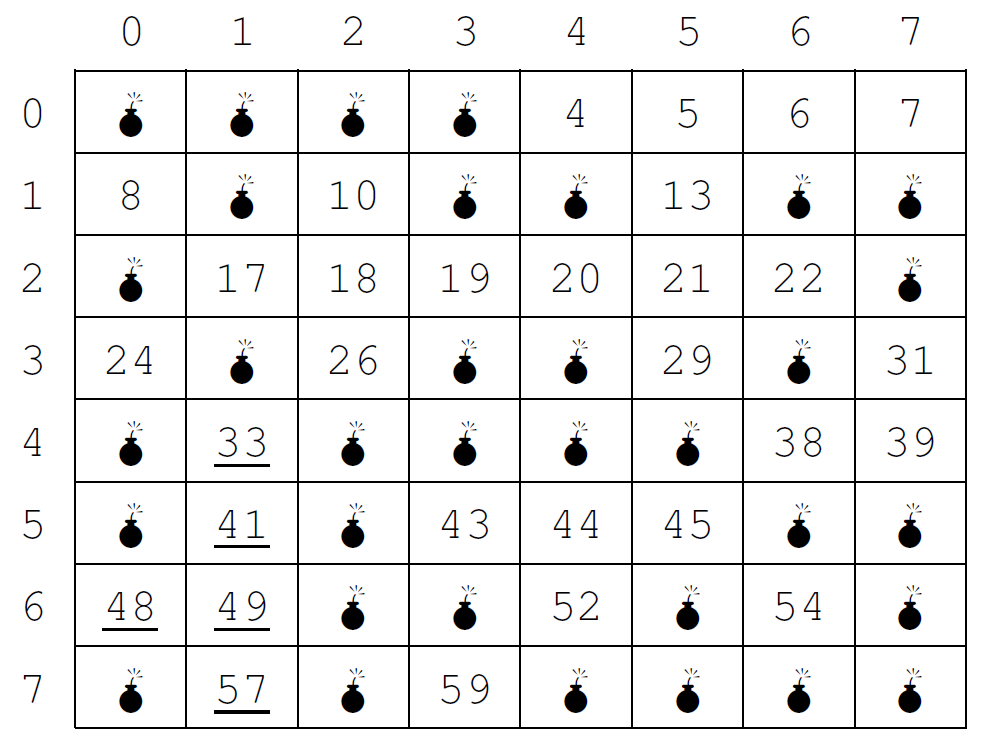
\includegraphics[scale=0.2]{Fig4-5.png}
		\end{column}
		\begin{column}{0.4\linewidth}
			\begin{figure}
				\animategraphics[scale=0.3,autoplay]{1}{example4_5/example4_5-}{1}{5}
			\end{figure}
		\end{column}
	\end{columns}
\end{frame}

\begin{frame}[fragile]
	\frametitle{4.6 \texttt{vector}类型\small{—使用迭代器}}
	% \framesubtitle{——使用迭代器}
	\begin{exampleblock}{代码清单4.5,例4.5:}
		% \centering
		\begin{lstlisting}[numbers=left,numberstyle=\small,numbers=left,xleftmargin=2em,framexleftmargin=2em,basicstyle=\small\ttfamily]
using namespace std;
int main() {
    srand(0);
    constexpr int sz = 8;
    char map[sz][sz];
    for (auto &row : map)
        for(auto &col:row)//以0.5的概率设置地雷,使用条件表达式简化代码
            col = rand() % 100 < 50 ? '*' : '0';
    //打印地图,函数setw设置打印字符的宽度(见10.2.2节)
    for (int i = 0; i < sz; ++i) {
        for (int j = 0; j < sz; ++j) {
            if (map[i][j] == '*') cout <<setw(3)<< "*";
            else cout << setw(3) << i*sz+j;
        }
        cout << endl;
    }
            \end{lstlisting}\ttfamily

	\end{exampleblock}
\end{frame}

\begin{frame}[fragile]
	\frametitle{4.6 vector类型\small{—使用迭代器}}
	% \framesubtitle{——使用迭代器}

	\begin{exampleblock}{代码清单4.5,例4.5:}
		% \centering
		\begin{lstlisting}[numbers=left,numberstyle=\small,numbers=left,xleftmargin=2em,framexleftmargin=2em,firstnumber=17,basicstyle=\small\ttfamily]
int cell;
cout << "请输入选择的方格编号[0-" << sz*sz - 1 << "]:";
cin >> cell;
if (map[cell/sz][cell%sz] == '*') {
    cout << "选择的是地雷" << endl;
}else //容器nobomb存放未处理的方格编号,初始值为选择的方格编号
    vector<int> result, nobomb(1,cell);
    map[cell / sz][cell%sz] = '1';//标记该方格已经遍历
    do {//取出nobomb中第一个待处理的方格编号,找到与cell相邻的方格
        cell = nobomb.front();
    //neibor存放与cell相邻的4个方格编号,如果没有对应方格编号标记为-1
        int neibor[]={(cell/sz>0)?cell-sz:-1,(cell%sz>0)?cell-1:-1,
            (cell/sz<sz-1)?cell+sz:-1,(cell%sz<sz-1)?cell+1:-1};
            \end{lstlisting}\ttfamily

	\end{exampleblock}
\end{frame}

\begin{frame}[fragile]
	\frametitle{4.6 vector类型\small{—使用迭代器}}
	% \framesubtitle{——使用迭代器}

	\begin{exampleblock}{代码清单4.5,例4.5:}
		% \centering
		\begin{lstlisting}[numbers=left,numberstyle=\small,numbers=left,xleftmargin=2em,framexleftmargin=2em,firstnumber=30,basicstyle=\small\ttfamily]
        for (auto &k : neibor) //注意k!=-1必须放到逻辑与的左侧
            if (k != -1 && map[k/sz][k%sz] == '0'){
                nobomb.push_back(k);//所有与cell相邻的无雷方格放到nobomb中
                map[k/sz][k%sz] = '1';//标记该方格已经遍历过
            }
        }
        result.push_back(cell); //将处理完的方格编号cell放到result中
        nobomb.erase(nobomb.begin());//将cell从nobomb中移除
    } while (!nobomb.empty());
    for (auto i : result)
        cout << i << " ";
}
return 0;
}
            \end{lstlisting}\ttfamily

	\end{exampleblock}
\end{frame}

\section{枚举类型}

\begin{frame}[fragile]
	\frametitle{4.7 枚举类型\small{—定义枚举类型}}
	% \framesubtitle{——定义枚举类型}
	\begin{block}{定义枚举类型}
		\begin{itemize}
			\item 不限定作用域
			      \begin{lstlisting}[basicstyle=\small\ttfamily]
enum color{red, green, blue};
            \end{lstlisting}
			      三个枚举成员的作用域与枚举类型本身的作用域相同\\
			      \begin{lstlisting}[basicstyle=\small\ttfamily]
enum emotion{happy, calm, blue};//错误:枚举成员 blue 已经定义过
            \end{lstlisting}
			\item 限定作用域
			      \begin{lstlisting}[basicstyle=\small\ttfamily]
enum class stoplight{red, green,yellow};
color c = red; //正确,可以访问color 类型的枚举成员
stoplight a = red; //错误:stoplight 类型的枚举成员red在此不可访问
            \end{lstlisting}
			      \texttt{\textcolor[rgb]{0,0,1}{stoplight b = stoplight::red; //正确}}
		\end{itemize}
	\end{block}
\end{frame}

\begin{frame}[fragile]
	\frametitle{4.7 枚举类型\small{—定义枚举类型}}
	% \framesubtitle{——定义枚举类型}
	\begin{block}{定义枚举类型}
		每个枚举成员都有一个\alert{常量整数值},默认值从0开始,依次加1。也可以指定枚举成员的值:
		\begin{lstlisting}[basicstyle=\small\ttfamily]
enum class week{Sunday = 7, Monday = 1, Tuesday, Wednesday,Thursday, Friday, Saturday};
        \end{lstlisting}
		枚举类型\texttt{week}中成员\texttt{Sunday}值为7,\texttt{Monday}值为1,\texttt{Tuesday}值为2、\texttt{Wednesday}值为3,依次类推。
	\end{block}
\end{frame}

\begin{frame}[fragile]
	\frametitle{4.7 枚举类型\small{—使用枚举类型}}
	% \framesubtitle{——使用枚举类型}
	\begin{block}{使用枚举类型}
		编译器不会把一个整型值自动转换为枚举类型:
		\begin{lstlisting}[basicstyle=\small\ttfamily]
color c1 = 1;//错误:类型不匹配
        \end{lstlisting}
		要用强制类型转换将一个整型值转换为一个枚举常量:
		\begin{lstlisting}[basicstyle=\small\ttfamily]
color c2 = static_cast<color>(1);
        \end{lstlisting}
	\end{block}
\end{frame}

\begin{frame}[fragile]
	\frametitle{4.7 枚举类型\small{—使用枚举类型}}
	% \framesubtitle{——使用枚举类型}
	\begin{block}{用\texttt{switch}分支结构列举枚举成员}
		\begin{columns}
			\begin{column}[t]{0.48\linewidth}
				\begin{lstlisting}[basicstyle=\small\ttfamily]
stoplight l= stoplight::red;
switch (l){
case stoplight::red:
    cout << "stop!" << endl;
    break;
case stoplight::green:
    cout << "pass carefully" << endl;
    break;
                \end{lstlisting}
			\end{column}
			\hfill
			\begin{column}[t]{0.48\linewidth}
				\begin{lstlisting}[basicstyle=\small\ttfamily]
case stoplight::yellow:
    cout << "slow down" << endl;
    break;
default:
    cout << "light broken, call 122"<< endl;
break;
}
                \end{lstlisting}
			\end{column}
		\end{columns}
	\end{block}
\end{frame}

\begin{frame}[fragile]
	\frametitle{~~}
	\begin{center}
		\huge{本章结束}
	\end{center}
\end{frame}

\end{document}
